\documentclass[
	11pt,			% Tamaño de fuente (11pt)
	letterpaper,	% Tamaño del papel (carta)
    twoside			% Impresión por ambos lados
]{thesis_utfsm}

\usepackage{thesis_utfsm}   % Archivo de estilos 

%!TEX root = memoria.tex

%---------------------------------------------------------------------------
%%% CONFIGURACIÓN
%---------------------------------------------------------------------------
%
%%% CODIFICACIÓN DE CARACTERES
% Este documento está escrito usando caracteres Unicode (UTF8)
% Por lo que la siguiente línea es necesaria para reconocer los acentos
% y otros caracteres en español.
% Si ve caracteres extraños en el PDF (en Windows o MAC) pruebe 
% con alguna de estas líneas:
\usepackage[utf8x]{inputenc}    % *nix / Linux / MacOSX
%\usepackage[latin1]{inputenc}  % Windows (MacOSX)

\newcommand{\TheTitle}{%
    \Large AUTOMATIZACIÓN DE LA FISCALIZACIÓN DE LOS DERECHOS DE PROPIEDAD INTELECTUAL DE MÚSICA CHILENA EN RADIOEMISORAS ONLINE
}%
\newcommand{\TheAuthor}          {MARCELA ALEJANDRA VIDAL RAMÍREZ}
\newcommand{\TheGrade}           {INGENIERO CIVIL INFORMÁTICO} % Elegir "O" ó "A"
\newcommand{\TheCity}            {SANTIAGO}
\newcommand{\TheDate}            {XXXXXX 2017}
\newcommand{\TheAdvisor}         {MARCELO MENDOZA}
\newcommand{\TheCoAdvisor}       {JAVIER ROBLEDO}
%\newcommand{\TheScndCoAdvisor}   {SRTA. XXXXXXX XXXXXXXX X.} % Opcional

% Marca de agua, puede ser deshabilitada para impresión rápida AGUA
%\insertWatermark{figures/logousm_watermark.jpg}
%---------------------------------------------------------------------------


%---------------------------------------------------------------------------
%%% No editar (¡Ver licencia!) (MIT License, 2016)
%---------------------------------------------------------------------------
\hypersetup{  
    pdfinfo={  
        Subject={Memoria Departamento de Industria, UTFSM},
        Keywords={Memoria} {Departamento de Industrias} {UTFSM},
        Producer={JCR LaTeX Templates, http://www.rubin-de-celis.com/},
        Licence={http://www.rubin-de-celis.com/LICENSE},
        pdfpagemode=FullScreen,
        pdfmenubar=false,
        pdftoolbar=false
    }  
}
\hypersetup{  
    pdfinfo={  
        Title={\TheTitle},
        Author={\TheAuthor}
    }  
}
%---------------------------------------------------------------------------              % Configuración (Título, autor, etc.)
                            
                            

\makeatother                


% Generadores de texto 
\usepackage{blindtext}      % automated text generation
\usepackage{lipsum}         % automated text generation
\usepackage{verbatim} % comentarios
\usepackage[none]{hyphenat} % evita cortar palabras
\usepackage{booktabs} % tablas
\usepackage{multirow} % tablas
\usepackage{placeins} % tablas después de texto
\usepackage{float} % Posicionar tablas
\usepackage{algorithm}
\usepackage{algorithmic}
\floatname{algorithm}{Algoritmo}
\renewcommand{\listalgorithmname}{Lista de algoritmos}
\renewcommand{\algorithmicrequire}{\textbf{Entrada:}}
\renewcommand{\algorithmicensure}{\textbf{Salida:}}
\renewcommand{\algorithmicend}{\textbf{Fin}}
\renewcommand{\algorithmicif}{\textbf{Si}}
\renewcommand{\algorithmicthen}{\textbf{Entonces}}
\renewcommand{\algorithmicelse}{\textbf{Si no}}
\renewcommand{\algorithmicelsif}{\algorithmicelse,\ \algorithmicif}
\renewcommand{\algorithmicendif}{\algorithmicend\ \algorithmicif}
\renewcommand{\algorithmicfor}{\textbf{Para}}
\renewcommand{\algorithmicforall}{\textbf{para todo}}
\renewcommand{\algorithmicdo}{\textbf{Hacer}}
\renewcommand{\algorithmicendfor}{\algorithmicend\ \algorithmicfor}
\renewcommand{\algorithmicwhile}{\textbf{Mientras}}
\renewcommand{\algorithmicendwhile}{\algorithmicend\ \algorithmicwhile}
\renewcommand{\algorithmicloop}{\textbf{repetir}}
\renewcommand{\algorithmicendloop}{\algorithmicend\ \algorithmicloop}
\renewcommand{\algorithmicrepeat}{\textbf{Repetir}}
\renewcommand{\algorithmicuntil}{\textbf{hasta que}}
\renewcommand{\algorithmicprint}{\textbf{Imprimir}} 
\renewcommand{\algorithmicreturn}{\textbf{Devolver}} 
\renewcommand{\algorithmictrue}{\textbf{Cierto }} 
\renewcommand{\algorithmicfalse}{\textbf{Falso }} 
 % archivo de traducción para algoritmos

%---------------------------------------------------------------------------
% variables para el texto
\newcommand{\NumElemTablaComparativaAPIS}{XXXX}

%%%%%%%%%%%%%%%%%%%%%%%%%%%%%%%%%%%%%%%%%%%%%%%%%%%%%%%%%%%%
%	Documento
%%%%%%%%%%%%%%%%%%%%%%%%%%%%%%%%%%%%%%%%%%%%%%%%%%%%%%%%%%%%
\begin{document}
\sloppy 

\pagestyle{plain}           % Headers & Footers (Roman numbers)

%---------------------------------------------------------------------------
%%%%%%%%%%%%%%%%%%%%%%%%%%%%%%%%%%%%
%	Portada
%%%%%%%%%%%%%%%%%%%%%%%%%%%%%%%%%%%%
\insertFile{portada}        % Insertar archivo 'sections/portada.tex'.

%---------------------------------------------------------------------------
%%%%%%%%%%%%%%%%%%%%%%%%%%%%%%%%%%%%
%	Preámbulo (Front Matter)
%%%%%%%%%%%%%%%%%%%%%%%%%%%%%%%%%%%%
\frontmatter                % Important! (Do not delete or move!)

\begin{comment}
 \dedicatoria{%
    \emph{\huge Dedicatoria \dots}

    \vspace*{2cm}[Puede ocupar este espacio para escribir una 
    dedicatoria (opcional). Revise el archivo maestro
    \inlinecode{memoria.tex}]
}%


\section*{(AGRADECIMIENTOS) [Título es opcional] }
\insertFile[empty]{agradecimientos} % Insertar 'sections/agradecimientos.tex'.
\end{comment}

\section*{RESUMEN}
\insertFile[plain]{Resumen}     % Insertar 'sections/resumen.tex'.


\section*{ABSTRACT}
\insertFile[plain]{Abstract}    % Insertar 'sections/abstract.tex'.


%%% TABLA DE CONTENIDOS / FIGURAS / CUADROS
\begin{spacing}{1}      % Single space for TOC, LOF and LOT
    \tableofcontents\listoftables\listoffigures
\end{spacing}



%---------------------------------------------------------------------------
%%%%%%%%%%%%%%%%%%%%%%%%%%%%%%%%%%%%
%	Cuerpo Principal (Main Matter)
%%%%%%%%%%%%%%%%%%%%%%%%%%%%%%%%%%%%
\mainmatter             

\pagestyle{fancy}       % Headers & Footers (Arabic numbers)

% Incluir Capítulos
%!TEX root = ../memoria.tex

\thispagestyle{empty}

\chapter*{Glosario}
\addcontentsline{toc}{chapter}{Glosario}

\markboth{GLOSARIO}{}

\lipsum[1-4]

\newpage\null\thispagestyle{empty}\newpage



%!TEX root = ../memoria.tex

\chapter*{Introducción}
\addcontentsline{toc}{chapter}{Introducción}

\markboth{INTRODUCCIÓN}{}


Tras ocho años de discusión en el congreso, el 18 de abril de 2015 se publicó la ley 20810 donde se declara que “(…) las radioemisoras que operen concesiones de radiodifusión sonora, en su programación diaria deberán emitir al menos una quinta parte (20\%) de música nacional, medida sobre el total de canciones emitidas, distribuida durante la jornada diaria de transmisión de cada emisora” [Biblioteca Congreso Nacional de Chile. (2015). Fija porcentajes mínimos de emisión de música nacional y música de raíz folklórica oral, a la radio difusión chilena. 13 de junio, 2016, de Biblioteca Congreso Nacional de Chile Sitio web: ...] y desde entonces, las diversas radios del país se vieron en la necesidad de adecuar sus parillas de programación para cumplir con la nueva disposición.

\bigskip

Si bien esta propuesta fue promulgada con el fin de promover la diversidad y potenciar la industria musical chilena, se debe considerar que el único ente encargado de distribuir las ganancias a cada artista es la Sociedad Chilena de Derechos de Autor (SCD) que tiene por objetivo administrar derechos autorales generados por la utilización de obras musicales y fonogramas, vale decir, producciones musicales en cualquiera de sus formatos [http://scd.cl/ Sociedad Chilena de Derechos de Autor].

\bigskip

No obstante, muchos de los artistas asociados a la SCD confiesa no saber cómo se realiza la gestión del proceso de derechos de autor sobre sus canciones, es más, según un estudio realizado por Open Business [Open Business. (2013). Desafíos de la gestión colectiva en Chile. 12 de junio, 2016, de Open Business. Sitio web: http://openbusinesslatinamerica.org/2013/04/22/desafios-de-la-gestion-colectiva-en-chile/] “muchas veces el público, los usuarios o los mismos artistas, no saben con precisión en qué consiste el trabajo de esta entidad, especialmente en un país donde ésta posee gran notoriedad pública por temas que no se relacionan directamente con la gestión que ella realiza”. Esto conlleva a generar cierta incertidumbre en los artistas sobre sus ganancias, pues no es factible fiscalizar las más de 30 radioemisoras locales para determinar cuál es la cantidad de reproducciones de sus canciones y llevar un control de la emisión radial de sus obras.

\bigskip

Es por ello, que en este trabajo se realiza un análisis y diseño de una plataforma 
 que permita a los artistas chilenos llevar un control del uso de su música a nivel radial para revisar simultáneamente en diversas radioemisoras online.
 
\lipsum[1-4]
 
La estructura de la presente memoria es la siguiente:

\begin{itemize}
\item El capítulo 1 detalla la propuesta a desarrollar, las razones para hacerlo, y los objetivos que se desean cumplir con ello.

\item El capítulo 2 muestra una indagación en la literatura abarcando principalmente las metodologías que existen para el reconocimiento de canciones digitalizadas, y los servicios y/o algoritmos más conocidos.

\item El capítulo 3 presenta el diseño inicial, explicando la metodología para desarrollar la solución y detalla la forma en que se llevó a cabo la implementación del algoritmo de reconocimiento acústico.

\item En el capítulo 4 se señalan las tareas realizadas para comprobar el rendimiento de la plataforma.

\item El capítulo 5 muestra los resultados obtenidos tras llevar a cabo la etapa anterior, analizando los valores recopilados.

\item Para finalizar, la Concusión resume el trabajo presentado, se comprueba el cumplimiento de los objetivos planteados, y se identifican los posibles trabajos a futuro.
\end{itemize}

% \newpage\null\thispagestyle{empty}\newpage



%!TEX root = ../memoria.tex

\chapter{Definición del problema}

\section{Descripción} \label{sec:Descripcion}

En Chile, la Sociedad de Derechos de Autor es el ente que se encarga de administrar los derechos de propiedad intelectual generados por la utilización de obras y fonogramas musicales, por tanto, su gestión se encarga de determinar los ingresos que los artistas reciben por el uso de sus creaciones musicales. 
El modo de operar se basa en la Ley de Propiedad Intelectual, la cual dispone que todas las radios y canales de televisión deben entregar a la sociedad sus planillas de ejecución, que reúnen la información de cada obra que comunican a través de sus programaciones. 

\bigskip

Por su parte, la SCD señala que la distribución de los derechos se basa en “una muestra aleatoria estadística de aproximadamente 6 días de emisión por cada mes completo enviado por las radioemisoras. Adicionalmente a la muestra aplicada a este rubro de reparto, se incluyen las obras (canciones) difundidas los días 17,18 y 19 de septiembre y 24, 25 y 31 de diciembre de cada año” [ ...], apoyándose además del Software de reconocimiento de música Vericast de BMAT “que tiene como objetivo aumentar la información que es emitida por las radioemisoras que cuenta con señal online ” [...]

\bigskip

Cabe destacar que la licencia para el uso del software Vericast fue adquirida a partir de la convocatoria de licitación pública realizada por el Concejo Nacional de las Artes (CNCA), bajo el programa de Medición Radial, difundido por el gobierno de Chile para el fomento de la música nacional [.../]. De esta forma, la SCD se adjudicó el proyecto, proponiendo la contratación del servicio de Vericast, y la puesta en marcha de su implementación hasta finales del año 2016 [...] y cuyas características se señalan a continuación:


\begin{verbatim}

http://transparenciaactiva.cultura.gob.cl/uploads/marcoNormativo/ebf456ab89212ce3af3173b8f2ebd18c5fc3a123.pdf
PAg 3, las partes convienen… CUATRO]
\end{verbatim}
Y cuyo costo, ascendió a un total de \$290.850.000 pesos chilenos, de los cuales:
\begin{verbatim}[Transcribir: http://transparenciaactiva.cultura.gob.cl/uploads/marcoNormativo/ebf456ab89212ce3af3173b8f2ebd18c5fc3a123.pdf

PAg 3, las partes convienen… TERCERO]
\end{verbatim}

No obstante, el primer balance, tras un año de la promulgación de la ley, reveló ciertos problemas a los que se vieron enfrentados los actores de la industria. Algunos directores de radios establecieron que en algunas ocasiones se programaron artistas y bandas locales que no figuran en los registros de la SCD provocando que no fueran reconocidos por el sistema: “ Si bien hace algunos meses la SCD puso a disposición de las radios una base de datos digitalizada de música nacional, con el fin de complementar catálogos -en especial para las radios regionales-, el problema persiste y con esto muchas veces las cifras del organismo no cuadran con los balances internos de cada señal.   ”[... ]

\bigskip

Los dos elementos que contribuyen a este escenario es que, por un lado, (explicar del encargado de la SCD, estipulado por licitación). Adicionalmente, existe un gran número de artistas que no se encuentran asociados a los registros de las SCD, tales como (buscar y nombrar artistas independientes).

\bigskip

Es en base a esta situación que surge la idea de diseñar y desarrollar una plataforma nacional que permita fiscalizar las más de 30 radioemisoras locales y comprobar de manera automática las parrillas musicales de cada una de éstas, permitiendo también, a los artistas chilenos no asociados a la SCD, llevar un control del uso de su música a nivel radial.


\section{Objetivos}

\subsection{Objetivo general} \label{sec:ObjetivoPrim}
\begin{itemize}
\item Detectar la frecuencia de reproducción de canciones de artistas chilenos en radioemisoras online.
\end{itemize}

\subsection{Objetivos secundarios} \label{sec:ObjetivosSec}
\begin{itemize}
\item Almacenar un catálogo de prueba de canciones nacionales en una base de datos.
\item Diseñar e implementar sistema de reconocimiento acústico para analizar en paralelo un conjunto de radioemisoras online.
\item Implementación de radioemisoras para validar solución desarrollada.
\end{itemize}
\section{Alcances} \label{sec:Alcances}
\lipsum[1-2]
%!TEX root = ../memoria.tex

\chapter{Estado del arte}
Dado que la principal funcionalidad a desarrollar para esta memoria decae en el reconocimiento y tratamiento de archivos de audio, para su comparación y análisis, se estudió en primera instancia sobre el modo de operación de algunas aplicaciones móviles conocidas que permiten reconocer audio a partir de comparaciones con el catálogo de canciones de su base de datos. 

\bigskip

Este análisis permitió comprender que dichas aplicaciones basan su funcionamiento en la espectrografía, disciplina que se dedica a medir la frecuencia de los sonidos en un determinado espacio de tiempo. De esta forma, un fragmento de música puede ser representado como una gráfica de frecuencias llamadas espectrogramas, donde en un eje, se observa el tiempo, en otro la frecuencia; y en algunos casos, un tercer eje representa la intensidad del sonido.


\section{Fiscalización de derechos de propiedad intelectual}
\lipsum[2-4]

\subsection{Content ID}
Sistema que escanea vídeos de YouTube y, si encuentra contenido con derechos –música, imagen, etcétera– notifica tanto al usuario como al poseedor legal del contenido.
Actually licensed from a company called Audible Magic: http://www.audiblemagic.com/ [7]


\subsection{Monitec}
Comercialización de herramientas tecnológicas para la captura, reconocimiento y monitoreo de medios electrónicos y acústicos. Utiliza huellas o patrones digitales de las canciones y anuncios publicitarios que se quieren detectar y las utiliza como base para recorrer, en tiempo real, la señal de radio o televisión que captan sus antenas.

\bigskip

El sistema de monitoreo musical y publicitario de Monitec ofrece un software diseñado especialmente para uso de la industria discográfica, industria publicitaria, medios de comunicación y sociedades de gestión colectiva. Monitoreo de Publicidad: Control de Pauta detallado, con el conteo y el detalle exacto de las apariciones de su cuña o spot publicitario en cada medio, ya sea este radio, televisión abierta o televisión por cable.


\subsection{Vericast}
Vericast es un servicio de BMAT (España) global de identificación de música que monitoriza millones de canciones en aproximadamente 3000 radios y televisiones de más de 60 países.

\bigskip

La solución ofrece una identificación a tiempo real y reportes auditables basados en la huella digital o fingerprint del audio que es resistente a alteraciones de la señal como en un canal degradado o ruidoso, cuando la música se utilice de fondo.
Bmat opera globalmente con más de 50 clientes en Europa [9], América y Asia. En 2011 incrementó sustancialmente sus ingresos respecto a 2010 y alcanzó los 1,1 millones de euros. Este año tienen previsto cerrar con 1,6 millones. Actualmente comercializa tres líneas de productos en una tecnología protegida por varias patentes internacionales.


\section{Algoritmos de reconocimiento acústico}

La principal metodología para la recuperación y reconocimiento de audio se basa en la huella digital acústica extraída de la canción en cuestión, la cual puede consistir en una muestra uniforme, o un resumen de los puntos de interés del espectrograma. 
Posteriormente, la información es comparada con una base de datos que consta de un catálogo de pistas de referencia para encontrar los mejores candidatos coincidentes. 
Sin embargo, para evitar hacer una comparación con todas las pistas de la base de datos, ésta puede ser particionada por Hash Directo, Locality Sensitive Hashing, u otras técnicas que se basan en la cuantización de vectores utilizados principalmente en datos comprimidos. De esta forma, es posible realizar una búsqueda más exacta en base a la vecindad de la solución [K. Mikolajczyk and C. Schmid. Performance evaluation of local descriptors. IEEE Transactions on Pattern Analysis and Machine Intelligence, 1615– 1630, 2005.].
Finalmente se realiza un último paso que permite tratar las coincidencias entregadas por la consulta de tal forma de eliminar de la respuesta los falsos positivos. 


\subsection{Paper 1}
\lipsum[2-4]

\section{Sistemas de reconocimiento acústico}


\subsection{Echoprint}
Open source music identification system that allows anyone to build music fingerprinting into their application. It is powered by The Echo Nest.

\subsection{ACRCloud}
El servicio de reconocimiento de música ACRCloud ofrece acceso a una de las bases de datos de huellas de audio digitales más grande del mundo con uno de los mejores índices de reconocimiento de la indústria.
Además, hemos integrado tecnologías de otros servicios musicales como Spotify, Deezer, iTunes, etc en nuestros resultados de reconocimiento, permitiendo a los desarrolladores proporcionar enlaces directos de estos servicios a sus usuarios, por ejemplo, para reproducir o comprar canciones inmediatamente.




\subsection{Echonest}
\lipsum[2-4]

\subsection{Dejavu project}
Audio fingerprinting and recognition algorithm implemented in Python.

Dejavu can memorize audio by listening to it once and fingerprinting it. Then by playing a song and recording microphone input, Dejavu attempts to match the audio against the fingerprints held in the database, returning the song being played


\subsection{Chromaprint}
Chromaprint is the core component of the AcoustID project. It's a client-side library that implements a custom algorithm for extracting fingerprints from any audio source.

Note that the library only calculates audio fingerprints from the provided raw uncompressed audio data. It does not deal with audio file formats in any way. Your application needs to find a way to decode audio files (MP3, MP4, FLAC, etc.) and feed the uncompressed data to Chromaprint.



\input{includes/DiseñoDeLaSolucion}
%!TEX root = ../memoria.tex

\chapter{Experimentos}

\section{Características del equipo}

\section{Implementación}
%!TEX root = ../memoria.tex

\chapter{Resultados}

\lipsum[1-8]

%!TEX root = ../memoria.tex


\chapter*{Conclusiones}
\addcontentsline{toc}{chapter}{Conclusiones}

\markboth{CONCLUSIONES}{}

\lipsum[1-4]

\newpage\null\thispagestyle{empty}\newpage



%!TEX root = ../memoria.tex

\chapter{Figuras}

\section{1}

%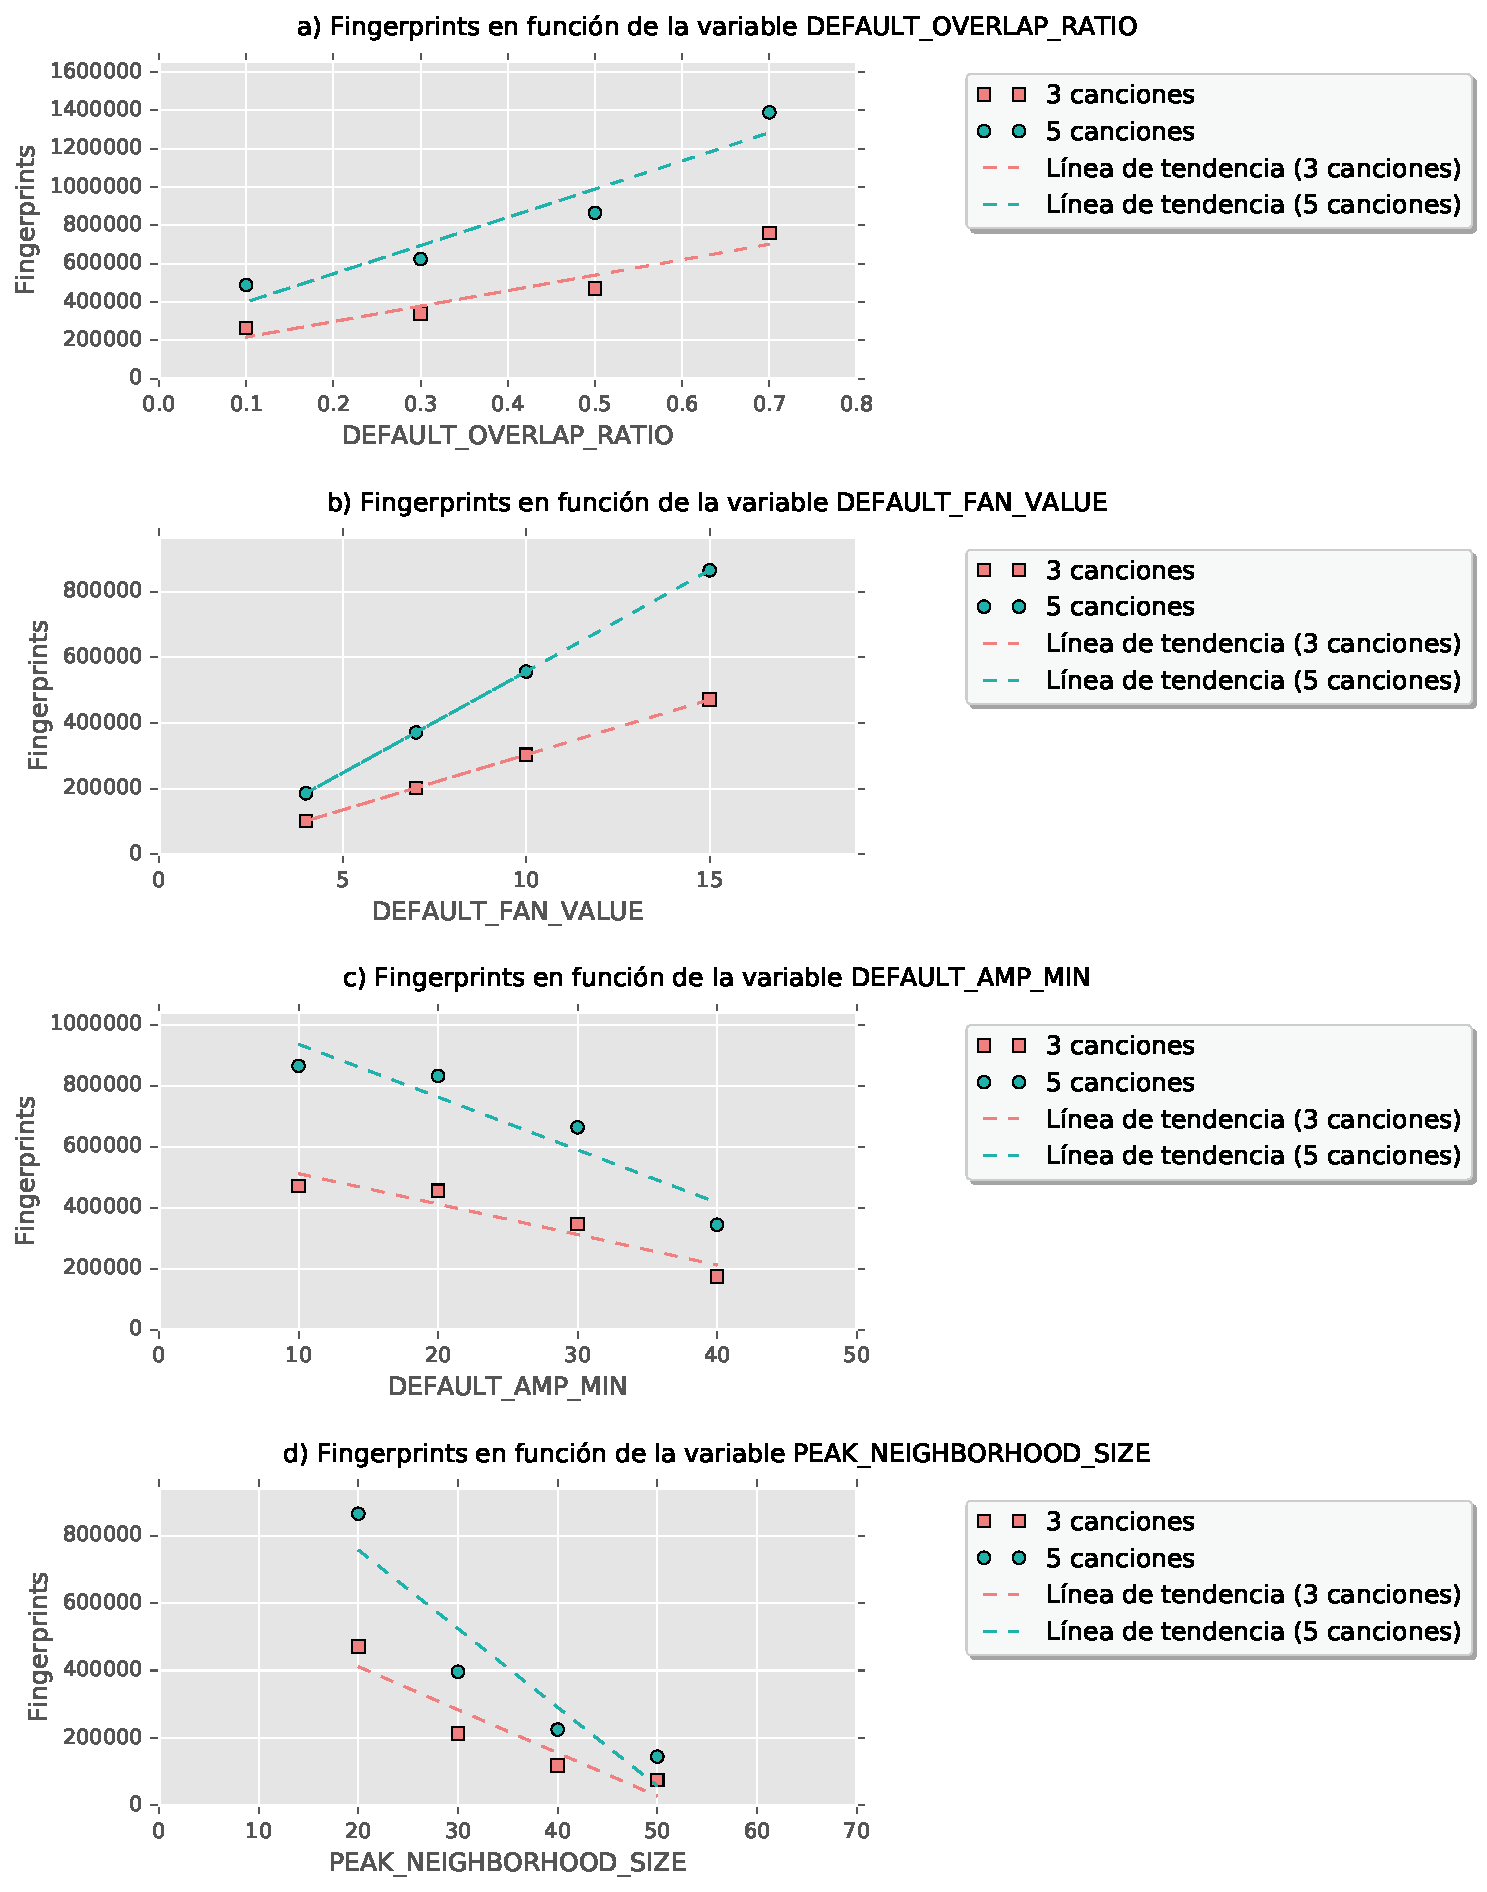
\includepdf[pages=-]{graficos/FingerprintsEnFuncionVariables.pdf}








\begin{figure}[h]
    \centering
    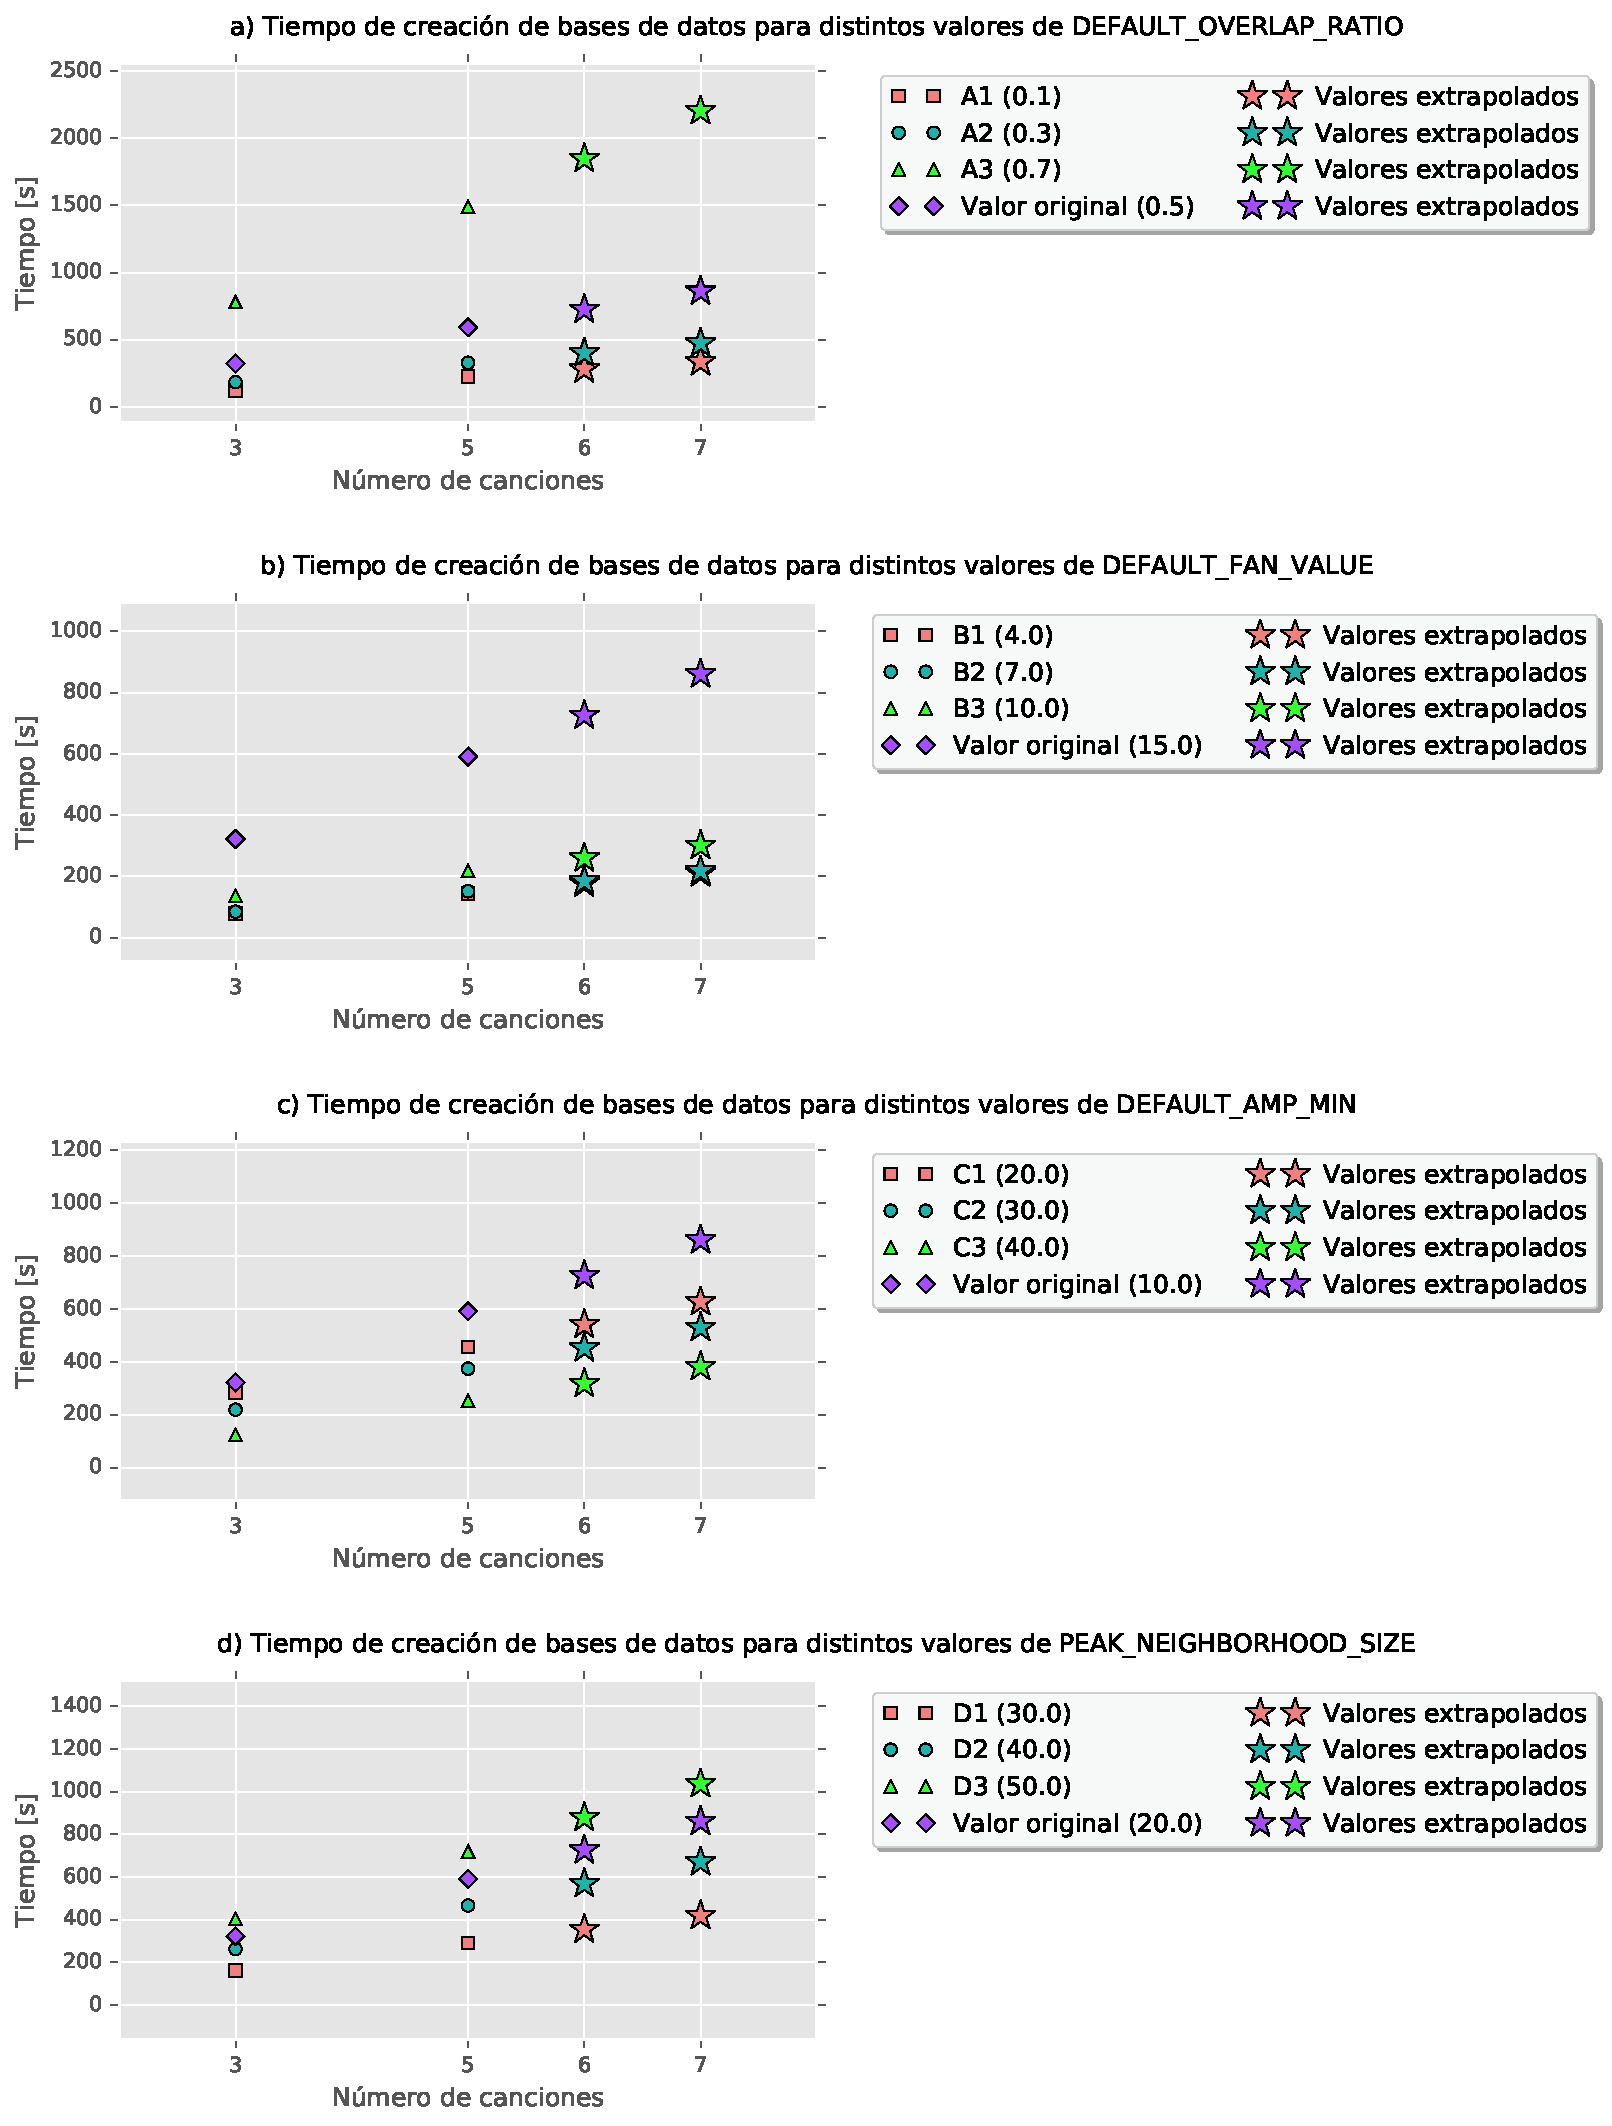
\includegraphics[scale=0.6]{graficos/AnalisisTest35Canciones.pdf}
    \caption{Tiempo de creación de bases de datos al modificar valores de configuración.}{Tiempo transcurrido en la creación de las bases de datos de tres y cinco canciones, con dos valores extrapolados para cada grupo de variables, utilizados para estimar cuanto tardaría una base de datos de 80.000 canciones.}
    \label{fig:AnalisisTest35Canciones}
\end{figure}
Mira mira \ref{fig:AnalisisTest35Canciones}

\begin{figure}[h]
    \centering
    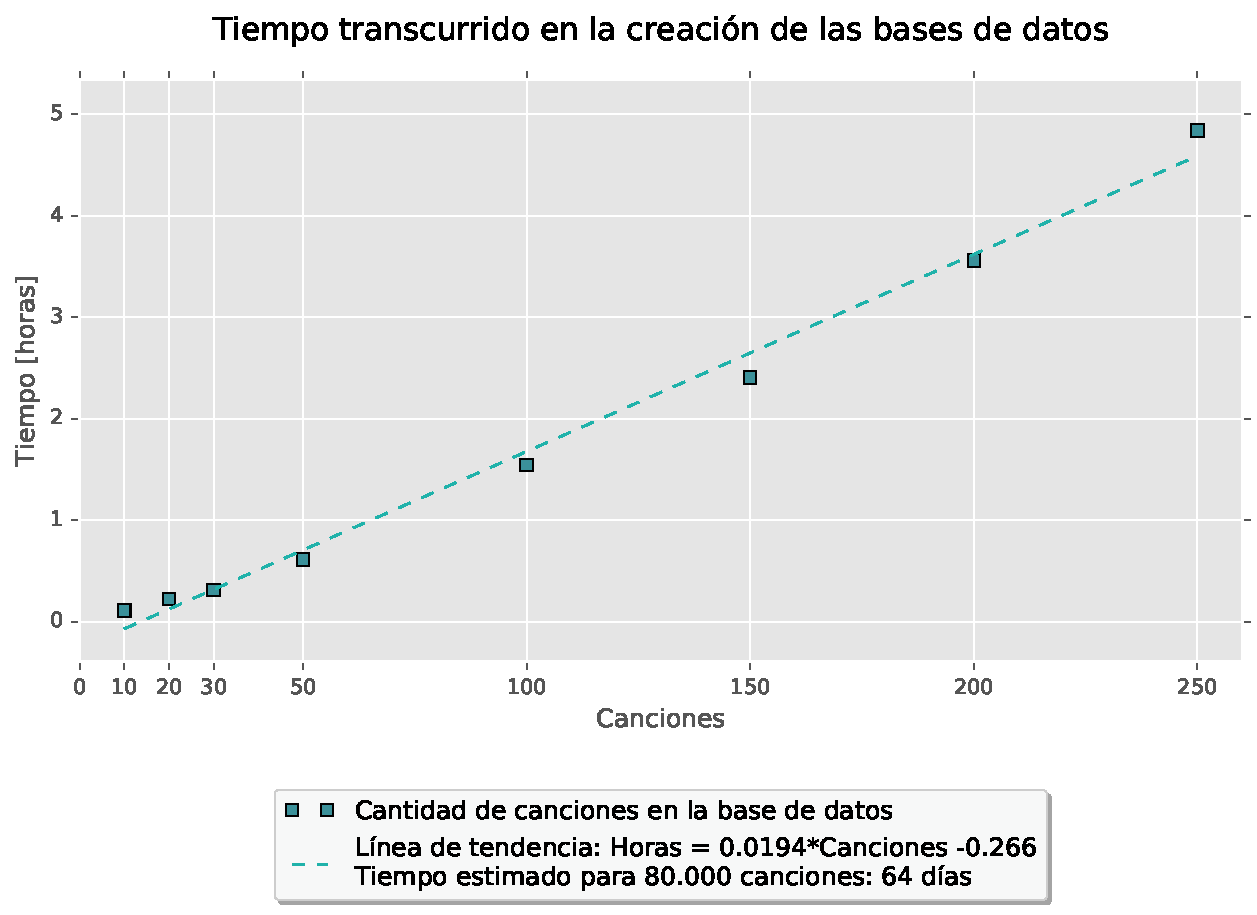
\includegraphics[scale=0.6]{graficos/ExtrapolarTiempoValoresConfiguracion.pdf}
    \caption{Tiempo en función del número de canciones de la nueva configuración de Dejavu.}{Tiempo transcurrido en la creación de las bases de datos con la nueva configuración de Dejavu. La ecuación de la línea de tendencia, permite extrapolar el valor de los días necesarios para crear la base de datos de 80.000 canciones de la plataforma.}
    \label{fig:ExtrapolarTiempoValoresConfiguracion}
\end{figure}
Mira mira \ref{fig:ExtrapolarTiempoValoresConfiguracion}


Mira mira \ref{fig:TiempoFingerprintOriginales}


%!TEX root = ../memoria.tex

\chapter{Tablas}

\section{1}


\FloatBarrier
\begin{table}[]
\centering
\caption{Valores originales de los parámetros de Dejavu.}
\label{tab:ConfiguracionBDDF35}
\begin{tabular}{@{}lrr@{}}
\toprule
\midrule
\multicolumn{1}{c}{Parámetro} & \multicolumn{1}{c}{F3\_3} & \multicolumn{1}{c}{F3\_5} \\ \midrule
DEFAULT\_OVERLAP\_RATIO   & 0,5                       & 0,5                       \\
DEFAULT\_FAN\_VALUE       & 15                        & 15                        \\
DEFAULT\_AMP\_MIN         & 10                        & 10                        \\
PEAK\_NEIGHBORHOOD\_SIZE  & 20                        & 20                        \\
PEAK\_SORT                & True                      & True                      \\
\midrule
Segundos                  & 322                       & 591                       \\
Fingerprints              & 470.938                   & 865.039                   \\
Tamaño {[}MB{]}           & 43,16                     & 82,25                     \\ \midrule \bottomrule
\end{tabular}
\end{table}


\begin{table}[]
\centering
\caption{Tiempo de creación de bases de datos, con los valores originales de Dejavu.}
\label{tab:TiemposOriginales}
\begin{tabular}{@{}crrr@{}}
\toprule
\midrule
\multicolumn{1}{l}{Número de canciones} & \multicolumn{1}{l}{Tiempo {[}seg{]}} & \multicolumn{1}{l}{Tiempo {[}min{]}} & \multicolumn{1}{l}{Tiempo {[}hr{]}} \\ \midrule
3                                       & 322                                  & 5,4                                  & 0,1                                 \\
5                                       & 591                                  & 9,9                                  & 0,2                                 \\
10                                      & 2.448                                & 40,8                                 & 0,7                                 \\
50                                      & 11.411                               & 190,2                                & 3,2                                 \\
100                                     & 24.938                               & 415,6                                & 6,9                                 \\
150                                     & 39.689                               & 661,5                                & 11,0                                \\
200                                     & 59.094                               & 984,9                                & 16,4                                \\
250                                     & 73.706                               & 1.228,4                              & 20,5                                
\\ \midrule \bottomrule
\end{tabular}
\end{table}




\begin{table}[]
\centering
\caption{Tiempo de creación de bases de datos, con los valores de configuración.}
\label{tab:TiemposNuevaConfiguracion}
\begin{tabular}{@{}crrr@{}}
\toprule
\midrule
\multicolumn{1}{l}{Número de canciones} & \multicolumn{1}{l}{Tiempo {[}seg{]}} & \multicolumn{1}{l}{Tiempo {[}min{]}} & \multicolumn{1}{l}{Tiempo {[}hr{]}} \\ \midrule
10                                      & 396                                & 6,6                                  & 0,1                                 \\
20                                      & 802                                & 13,4                                 & 0,2                                 \\
30                                      & 1124                               & 18,7                                 & 0,3                                 \\
50                                      & 2206                               & 36,8                                 & 0,6                                 \\
100                                     & 5555                               & 92,6                                 & 1,5                                 \\
150                                     & 8666                               & 144,4                                & 2,4                                 \\
200                                     & 12821                              & 213,7                                & 3,6                                 \\
250                                     & 17428                              & 290,5                                & 4,8                                 \\
\midrule \bottomrule
\end{tabular}
\end{table}


\begin{table}[]
\centering
\caption{Valores de configuración de las bases de datos de 3 y 5 canciones.}{La tabla señala las 26 bases de datos para las cuales se modifica un solo parámetro de configuración, con sus respectivos tiempos de creación, cantidad de fingerprints y tamaño.}
\label{tab:ConfiguracionBDD35}
\begin{tabular}{@{}ccrrrr@{}}
\toprule
\midrule
Bases de datos & Variable modificada                       & \multicolumn{1}{c}{Valor} & \multicolumn{1}{c}{Segundos} & \multicolumn{1}{c}{Fingerprints} & \multicolumn{1}{c}{Tamaño {[}MB{]}} \\ \midrule
A1\_3          & \multirow{6}{*}{DEFAULT\_OVERLAP\_RATIO}  & 0,10                      & 118                          & 264.963                          & 26,09                               \\
A1\_5          &                                           & 0,10                      & 226                          & 488.378                          & 47,17                               \\
A2\_3          &                                           & 0,30                      & 183                          & 340.149                          & 30,11                               \\
A2\_5          &                                           & 0,30                      & 328                          & 623.970                          & 58,19                               \\
A3\_3          &                                           & 0,70                      & 779                          & 760.517                          & 66,22                               \\
A3\_5          &                                           & 0,70                      & 1492                         & 1.389.934                        & 119,31                              \\\midrule
B1\_3          & \multirow{6}{*}{DEFAULT\_FAN\_VALUE}      & 4                         & 78                           & 101.020                          & 11,06                               \\
B1\_5          &                                           & 4                         & 144                          & 185.543                          & 19,09                               \\
B2\_3          &                                           & 7                         & 85                           & 202.019                          & 21,09                               \\
B2\_5          &                                           & 7                         & 151                          & 371.056                          & 37,16                               \\
B3\_3          &                                           & 10                        & 137                          & 302.977                          & 27,11                               \\
B3\_5          &                                           & 10                        & 218                          & 556.456                          & 48,17                               \\
\midrule
C1\_3          & \multirow{6}{*}{DEFAULT\_AMP\_MIN}        & 20                        & 284                          & 455.623                          & 41,16                               \\
C1\_5          &                                           & 20                        & 455                          & 831.922                          & 84,25                               \\
C2\_3          &                                           & 30                        & 219                          & 346.760                          & 30,11                               \\
C2\_5          &                                           & 30                        & 374                          & 663.643                          & 56,19                               \\
C3\_3          &                                           & 40                        & 125                          & 174.205                          & 17,06                               \\
C3\_5          &                                           & 40                        & 253                          & 344.135                          & 31,11                               \\
\midrule
D1\_3          & \multirow{6}{*}{PEAK\_NEIGHBORHOOD\_SIZE} & 30                        & 162                          & 213.056                          & 21,09                               \\
D1\_5          &                                           & 30                        & 290                          & 396.462                          & 38,14                               \\
D2\_3          &                                           & 40                        & 262                          & 118.504                          & 13,06                               \\
D2\_5          &                                           & 40                        & 466                          & 224.778                          & 23,09                               \\
D3\_3          &                                           & 50                        & 404                          & 75.614                           & 7,06                                \\
D3\_5          &                                           & 50                        & 720                          & 144.452                          & 14,06                               \\
\midrule
E1\_3          & \multirow{2}{*}{PEAK\_SORT}               & FALSE                     & 100                          & 24.725                           & 3,06                                \\
E1\_5          &                                           & FALSE                     & 240                          & 46.162                           & 6,06                                \\
\midrule
\bottomrule
\end{tabular}
\end{table}





\begin{sidewaystable}
\centering
\caption{Resumen de los resultados de Dejavu al probar 27 extractos de música.}{Las pruebas se realizaron con cada base de datos que solo contiene 3 canciones, generando extractos de 5,10, y 15 segundos para realizar el reconocimiento acústico.}
\label{tab:Resumen3Canciones}
\begin{tabular}{@{}ccc|rrrrrrrrrrrrrr@{}}
\toprule
\midrule
\multicolumn{2}{c}{Salida}                                            &  Segundos  & \multicolumn{1}{c}{A1} & \multicolumn{1}{c}{A2} & \multicolumn{1}{c}{A3} & \multicolumn{1}{c}{B1} & \multicolumn{1}{c}{B2} & \multicolumn{1}{c}{B3} & \multicolumn{1}{c}{C1} & \multicolumn{1}{c}{C2} & \multicolumn{1}{c}{C3} & \multicolumn{1}{c}{D1} & \multicolumn{1}{c}{D2} & \multicolumn{1}{c}{D3} & \multicolumn{1}{c}{E1} & \multicolumn{1}{c}{F1} \\ \midrule
\multirow{6}{*}{Respuesta Dejavu}    & \multirow{3}{*}{Aciertos}   & 5  & 9                      & 9                      & 9                      & 9                      & 8                      & 8                      & 8                      & 8                      & 8                      & 8                      & 8                      & 8                      & 2                      & 8                      \\
                                     &                             & 10 & 9                      & 9                      & 9                      & 9                      & 9                      & 9                      & 9                      & 9                      & 9                      & 9                      & 9                      & 9                      & 1                      & 9                      \\
                                     &                             & 15 & 9                      & 9                      & 9                      & 9                      & 9                      & 9                      & 9                      & 9                      & 9                      & 9                      & 9                      & 9                      & 3                      & 9                      \\ \cmidrule{2-17}
                                     & \multirow{3}{*}{Errores}    & 5  & 0                      & 0                      & 0                      & 0                      & 1                      & 1                      & 1                      & 1                      & 1                      & 1                      & 1                      & 0                      & 0                      & 1                      \\ 
                                     &                             & 10 & 0                      & 0                      & 0                      & 0                      & 0                      & 0                      & 0                      & 0                      & 0                      & 0                      & 0                      & 0                      & 0                      & 0                      \\
                                     &                             & 15 & 0                      & 0                      & 0                      & 0                      & 0                      & 0                      & 0                      & 0                      & 0                      & 0                      & 0                      & 0                      & 0                      & 0                      \\
\midrule
\multicolumn{2}{c}{\multirow{3}{*}{Sin respuesta}}                 & 5  & 0                      & 0                      & 0                      & 0                      & 0                      & 0                      & 0                      & 0                      & 0                      & 0                      & 0                      & 1                      & 7                      & 0                      \\
\multicolumn{2}{c}{}                                               & 10 & 0                      & 0                      & 0                      & 0                      & 0                      & 0                      & 0                      & 0                      & 0                      & 0                      & 0                      & 0                      & 8                      & 0                      \\
\multicolumn{2}{c}{}                                               & 15 & 0                      & 0                      & 0                      & 0                      & 0                      & 0                      & 0                      & 0                      & 0                      & 0                      & 0                      & 0                      & 6                      & 0                      \\
\midrule
\multicolumn{2}{c}{\multirow{3}{*}{Tiempo mínimo de búsqueda {[}seg{]}}}     & 5  & 1                      & 1                      & 4                      & 1                      & 1                      & 1                      & 1                      & 1                      & 1                      & 1                      & 1                      & 1                      & 3                      & 3                      \\
\multicolumn{2}{c}{}                                               & 10 & 2                      & 3                      & 9                      & 2                      & 2                      & 2                      & 3                      & 2                      & 2                      & 2                      & 2                      & 2                      & 3                      & 8                      \\
\multicolumn{2}{c}{}                                               & 15 & 3                      & 4                      & 14                     & 3                      & 3                      & 3                      & 5                      & 4                      & 3                      & 3                      & 3                      & 1                      & 10                     & 13                     \\
\midrule
\multicolumn{2}{c}{\multirow{3}{*}{Tiempo máximo de búsqueda {[}seg{]}}}     & 5  & 4                      & 1                      & 6                      & 1                      & 1                      & 1                      & 2                      & 2                      & 1                      & 1                      & 1                      & 2                      & 11                     & 5                      \\
\multicolumn{2}{c}{}                                               & 10 & 7                      & 3                      & 12                     & 2                      & 2                      & 2                      & 5                      & 3                      & 2                      & 2                      & 2                      & 3                      & 7                      & 11                     \\
\multicolumn{2}{c}{}                                               & 15 & 11                     & 5                      & 18                     & 3                      & 3                      & 3                      & 8                      & 6                      & 3                      & 3                      & 3                      & 3                      & 11                     & 16                     \\
\midrule
\multicolumn{2}{c}{\multirow{3}{*}{Confidencia mínima (aciertos)}} & 5  & 1                      & 3                      & 1                      & 1                      & 39                     & 56                     & 78                     & 39                     & 2                      & 30                     & 10                     & 5                      & 1                      & 78                     \\
\multicolumn{2}{c}{}                                               & 10 & 7                      & 15                     & 20                     & 24                     & 42                     & 71                     & 87                     & 43                     & 18                     & 24                     & 9                      & 3                      & 3                      & 88                     \\
\multicolumn{2}{c}{}                                               & 15 & 7                      & 15                     & 20                     & 68                     & 126                    & 179                    & 243                    & 215                    & 62                     & 89                     & 29                     & 20                     & 1                      & 243                    \\
\midrule
\multicolumn{2}{c}{\multirow{3}{*}{Confidencia máxima (errores)}}  & 5  & -                      & -                      & -                      & -                      & 1                      & 1                      & 1                      & 1                      & 1                      & 1                      & 1                      & -                      & -                      & 1                      \\
\multicolumn{2}{c}{}                                               & 10 & -                      & -                      & -                      & -                      & -                      & -                      & -                      & -                      & -                      & -                      & -                      & -                      & -                      & -                      \\
\multicolumn{2}{c}{}                                               & 15 & -                      & -                      & -                      & -                      & -                      & -                      & -                      & -                      & -                      & -                      & -                      & -                      & -                      & -                      \\
\midrule
\multicolumn{2}{c}{Días estimados para la creación de 80000 canciones}         &    & 100                    & 134                    & 660                    & 62                     & 62                     & 76                     & 158                    & 328                    & 118                    & 248                    & 436                    & 660                    &                        & 250                    \\ \midrule \bottomrule
\end{tabular}
\end{sidewaystable}





\begin{sidewaystable}
\centering
\caption{Resumen de los resultados de Dejavu al probar 18 extractos de música.}{Los extractos de 5, 10, y 15 segundos, se generan de 2 canciones aleatorias que no son parte de las bases de datos.}
\label{tab:Resumen3SinCanciones}
\begin{tabular}{@{}ccc|rrrrrrrrrrrrrr@{}}
\toprule
\midrule
\multicolumn{2}{c}{Salida}                                            &  Segundos  & \multicolumn{1}{c}{A1} & \multicolumn{1}{c}{A2} & \multicolumn{1}{c}{A3} & \multicolumn{1}{c}{B1} & \multicolumn{1}{c}{B2} & \multicolumn{1}{c}{B3} & \multicolumn{1}{c}{C1} & \multicolumn{1}{c}{C2} & \multicolumn{1}{c}{C3} & \multicolumn{1}{c}{D1} & \multicolumn{1}{c}{D2} & \multicolumn{1}{c}{D3} & \multicolumn{1}{c}{E1} & \multicolumn{1}{c}{F1} \\ \midrule

\multirow{6}{*}{Respuesta Dejavu}   & \multirow{3}{*}{Aciertos}  & 5                    & 0                      & 0                      & 0                      & 0                      & 0                      & 0                      & 0                      & 0                      & 0                      & 0                      & 0                      & 0                      & 0                      & 0                      \\
                                      &                            & 10                   & 0                      & 0                      & 0                      & 0                      & 0                      & 0                      & 0                      & 0                      & 0                      & 0                      & 0                      & 0                      & 0                      & 0                      \\
                                      &                            & 15                   & 0                      & 0                      & 0                      & 0                      & 0                      & 0                      & 0                      & 0                      & 0                      & 0                      & 0                      & 0                      & 0                      & 0                      \\ \cmidrule{2-17}
                                      & \multirow{3}{*}{Errores}   & 5                    & 6                      & 6                      & 6                      & 6                      & 6                      & 6                      & 6                      & 6                      & 6                      & 6                      & 5                      & 5                      & 0                      & 6                      \\
                                      &                            & 10                   & 6                      & 6                      & 6                      & 6                      & 6                      & 6                      & 6                      & 6                      & 6                      & 6                      & 6                      & 6                      & 0                      & 6                      \\
                                      &                            & 15                   & 6                      & 6                      & 6                      & 6                      & 6                      & 6                      & 6                      & 6                      & 6                      & 6                      & 6                      & 6                      & 0                      & 6                      \\
\midrule
\multicolumn{2}{c}{\multirow{3}{*}{Sin Respuesta}}            & 5                    & 0                      & 0                      & 0                      & 0                      & 0                      & 0                      & 0                      & 0                      & 0                      & 0                      & 1                      & 1                      & 6                      & 0                      \\
\multicolumn{2}{c}{}                                               & 10                   & 0                      & 0                      & 0                      & 0                      & 0                      & 0                      & 0                      & 0                      & 0                      & 0                      & 0                      & 0                      & 6                      & 0                      \\
\multicolumn{2}{c}{}                                               & 15                   & 0                      & 0                      & 0                      & 0                      & 0                      & 0                      & 0                      & 0                      & 0                      & 0                      & 0                      & 0                      & 6                      & 0                      \\
\midrule
\multicolumn{2}{c}{\multirow{3}{*}{Tiempo mínimo de búsqueda {[}seg{]}}}     & 5                    & -1                     & -1                     & -1                     & -1                     & -1                     & -1                     & -1                     & -1                     & -1                     & -1                     & -1                     & -1                     & -1                     & -1                     \\
\multicolumn{2}{c}{}                                               & 10                   & -1                     & -1                     & -1                     & -1                     & -1                     & -1                     & -1                     & -1                     & -1                     & -1                     & -1                     & -1                     & -1                     & -1                     \\
\multicolumn{2}{c}{}                                               & 15                   & -1                     & -1                     & -1                     & -1                     & -1                     & -1                     & -1                     & -1                     & -1                     & -1                     & -1                     & -1                     & -1                     & -1                     \\
\midrule
\multicolumn{2}{c}{\multirow{3}{*}{Tiempo máximo de búsqueda {[}seg{]}}}     & 5                    & 1                      & 1                      & 6                      & 1                      & 1                      & 1                      & 3                      & 2                      & 1                      & 1                      & 2                      & 2                      & -1                     & 6                      \\
\multicolumn{2}{c}{}                                               & 10                   & 2                      & 3                      & 12                     & 2                      & 2                      & 2                      & 5                      & 4                      & 2                      & 2                      & 3                      & 3                      & -1                     & 11                     \\
\multicolumn{2}{c}{}                                               & 15                   & 3                      & 5                      & 18                     & 3                      & 3                      & 3                      & 8                      & 6                      & 3                      & 3                      & 3                      & 3                      & -1                     & 17                     \\
\midrule
\multicolumn{2}{c}{\multirow{3}{*}{Confidencia mínima (aciertos)}} & 5                    & -                      & -                      & -                      & -                      & -                      & -                      & -                      & -                      & -                      & -                      & -                      & -                      & -                      & -                      \\
\multicolumn{2}{c}{}                                               & 10                   & -                      & -                      & -                      & -                      & -                      & -                      & -                      & -                      & -                      & -                      & -                      & -                      & -                      & -                      \\
\multicolumn{2}{c}{}                                               & 15                   & -                      & -                      & -                      & -                      & -                      & -                      & -                      & -                      & -                      & -                      & -                      & -                      & -                      & -                      \\
\midrule
\multicolumn{2}{c}{\multirow{3}{*}{Confidencia máxima (errores)}}  & 5                    & 3                      & 3                      & 3                      & 4                      & 4                      & 4                      & 4                      & 4                      & 3                      & 2                      & 2                      & 1                      & -                      & 4                      \\
\multicolumn{2}{c}{}                                               & 10                   & 4                      & 4                      & 4                      & 4                      & 4                      & 4                      & 4                      & 4                      & 3                      & 3                      & 2                      & 1                      & -                      & 4                      \\
\multicolumn{2}{c}{}                                               & 15                   & 4                      & 4                      & 6                      & 4                      & 4                      & 4                      & 4                      & 4                      & 3                      & 3                      & 3                      & 2                      & -                      & 4                      \\
\midrule
\multicolumn{2}{c}{Días estimados para la creación de 80000 canciones}         &                      & 100                    & 134                    & 660                    & 62                     & 62                     & 76                     & 158                    & 328                    & 118                    & 248                    & 436                    & 660                    &                        & 250                    \\ \midrule \bottomrule


\end{tabular}
\end{sidewaystable}

\begin{sidewaystable}
\centering
\caption{Resumen de los resultados de Dejavu al probar 45 extractos de música.}{Las pruebas se realizaron con cada base de datos que solo contiene 5 canciones, generando extractos de 5,10, y 15 segundos para realizar el reconocimiento acústico.}
\label{tab:Resumen5Canciones}
\begin{tabular}{@{}ccc|rrrrrrrrrrrrrr@{}}
\toprule
\midrule
\multicolumn{2}{c}{Salida}                                            &  Segundos  & \multicolumn{1}{c}{A1} & \multicolumn{1}{c}{A2} & \multicolumn{1}{c}{A3} & \multicolumn{1}{c}{B1} & \multicolumn{1}{c}{B2} & \multicolumn{1}{c}{B3} & \multicolumn{1}{c}{C1} & \multicolumn{1}{c}{C2} & \multicolumn{1}{c}{C3} & \multicolumn{1}{c}{D1} & \multicolumn{1}{c}{D2} & \multicolumn{1}{c}{D3} & \multicolumn{1}{c}{E1} & \multicolumn{1}{c}{F1} \\ \midrule


\multirow{6}{*}{Con reconocimiento}   & \multirow{3}{*}{Aciertos}  & 5                    & 14                     & 15                     & 15                     & 15                     & 14                     & 14                     & 14                     & 14                     & 12                     & 14                     & 14                     & 14                     & 3                      & 14                     \\
                                      &                            & 10                   & 15                     & 15                     & 15                     & 15                     & 15                     & 15                     & 15                     & 15                     & 15                     & 15                     & 15                     & 15                     & 3                      & 15                     \\
                                      &                            & 15                   & 15                     & 15                     & 15                     & 15                     & 15                     & 15                     & 15                     & 15                     & 15                     & 15                     & 15                     & 15                     & 4                      & 15                     \\ \cmidrule{2-17}
                                      & \multirow{3}{*}{Errores}   & 5                    & 1                      & 0                      & 0                      & 0                      & 1                      & 1                      & 1                      & 1                      & 3                      & 1                      & 1                      & 1                      & 0                      & 1                      \\
                                      &                            & 10                   & 0                      & 0                      & 0                      & 0                      & 0                      & 0                      & 0                      & 0                      & 0                      & 0                      & 0                      & 0                      & 0                      & 0                      \\
                                      &                            & 15                   & 0                      & 0                      & 0                      & 0                      & 0                      & 0                      & 0                      & 0                      & 0                      & 0                      & 0                      & 0                      & 0                      & 0                      \\
\midrule
\multicolumn{2}{c}{\multirow{3}{*}{Sin reconocimiento}}            & 5                    & 0                      & 0                      & 0                      & 0                      & 0                      & 0                      & 0                      & 0                      & 0                      & 0                      & 0                      & 0                      & 12                     & 0                      \\
\multicolumn{2}{c}{}                                               & 10                   & 0                      & 0                      & 0                      & 0                      & 0                      & 0                      & 0                      & 0                      & 0                      & 0                      & 0                      & 0                      & 12                     & 0                      \\
\multicolumn{2}{c}{}                                               & 15                   & 0                      & 0                      & 0                      & 0                      & 0                      & 0                      & 0                      & 0                      & 0                      & 0                      & 0                      & 0                      & 11                     & 0                      \\
\midrule
\multicolumn{2}{c}{\multirow{3}{*}{Tiempo mínimo de búsqueda {[}seg{]}}}     & 5                    & 1                      & 1                      & 4                      & 1                      & 1                      & 1                      & 1                      & 1                      & 3                      & 1                      & 1                      & 1                      & 3                      & 4                      \\
\multicolumn{2}{c}{}                                               & 10                   & 3                      & 3                      & 9                      & 2                      & 2                      & 3                      & 3                      & 3                      & 7                      & 3                      & 2                      & 2                      & 3                      & 9                      \\
\multicolumn{2}{c}{}                                               & 15                   & 5                      & 5                      & 14                     & 3                      & 5                      & 5                      & 6                      & 6                      & 12                     & 5                      & 3                      & 3                      & 11                     & 14                     \\
\midrule
\multicolumn{2}{c}{\multirow{3}{*}{Tiempo máximo de búsqueda {[}seg{]}}}     & 5                    & 3                      & 3                      & 7                      & 1                      & 2                      & 3                      & 3                      & 3                      & 5                      & 2                      & 1                      & 1                      & 11                     & 7                      \\
\multicolumn{2}{c}{}                                               & 10                   & 5                      & 5                      & 13                     & 2                      & 4                      & 5                      & 6                      & 5                      & 10                     & 5                      & 2                      & 2                      & 7                      & 13                     \\
\multicolumn{2}{c}{}                                               & 15                   & 9                      & 8                      & 19                     & 3                      & 7                      & 8                      & 9                      & 8                      & 15                     & 7                      & 3                      & 3                      & 11                     & 19                     \\
\midrule
\multicolumn{2}{c}{\multirow{3}{*}{Confidencia mínima (aciertos)}} & 5                    & 1                      & 2                      & 1                      & 1                      & 11                     & 15                     & 9                      & 3                      & 26                     & 4                      & 2                      & 1                      & 1                      & 19                     \\
\multicolumn{2}{c}{}                                               & 10                   & 7                      & 15                     & 19                     & 24                     & 42                     & 66                     & 87                     & 43                     & 18                     & 24                     & 7                      & 3                      & 2                      & 88                     \\
\multicolumn{2}{c}{}                                               & 15                   & 7                      & 15                     & 20                     & 43                     & 69                     & 104                    & 143                    & 109                    & 62                     & 31                     & 8                      & 4                      & 1                      & 138                    \\
\midrule
\multicolumn{2}{c}{\multirow{3}{*}{Confidencia máxima (errores)}}  & 5                    & 5                      & -                      & -                      & -                      & 1                      & 1                      & 1                      & 1                      & 3                      & 1                      & 1                      & 1                      & -                      & 1                      \\
\multicolumn{2}{c}{}                                               & 10                   & -                      & -                      & -                      & -                      & -                      & -                      & -                      & -                      & -                      & -                      & -                      & -                      & -                      & -                      \\
\multicolumn{2}{c}{}                                               & 15                   & -                      & -                      & -                      & -                      & -                      & -                      & -                      & -                      & -                      & -                      & -                      & -                      & -                      & -                      \\
\midrule
\multicolumn{2}{c}{Días estimados para la creación de 80000 canciones}          &                      & 100                    & 134                    & 660                    & 62                     & 62                     & 76                     & 158                    & 328                    & 118                    & 248                    & 436                    & 660                    &                        & 250                    \\ \midrule \bottomrule


\end{tabular}
\end{sidewaystable}


























\begin{sidewaystable}
\centering
\caption{Resumen de los resultados de Dejavu al probar 216 extractos de covers.}{Los extractos de 5, 10, y 15 segundos, se generan de 24 covers presentes en las bases de datos.}
\label{tab:ResumenCovers}
\begin{tabular}{@{}ccc|rrrrrr@{}}
\toprule
\midrule
\multicolumn{2}{c}{Salida}                                         & Segundos & \multicolumn{1}{c}{Covers30} & \multicolumn{1}{c}{Covers50} & \multicolumn{1}{c}{Covers100} & \multicolumn{1}{c}{Covers150} & \multicolumn{1}{c}{Covers200} & \multicolumn{1}{c}{Covers250} \\ \midrule
\multirow{6}{*}{Con reconocimiento}   & \multirow{3}{*}{Aciertos}  & 5        & 61                           & 61                           & 60                            & 60                            & 60                            & 60                            \\
                                      &                            & 10       & 71                           & 71                           & 71                            & 71                            & 71                            & 71                            \\
                                      &                            & 15       & 72                           & 72                           & 72                            & 72                            & 72                            & 72                            \\ \cmidrule{2-9}
                                      & \multirow{3}{*}{Errores}   & 5        & 4                            & 4                            & 5                             & 5                             & 5                             & 5                             \\
                                      &                            & 10       & 0                            & 0                            & 0                             & 0                             & 0                             & 0                             \\
                                      &                            & 15       & 0                            & 0                            & 0                             & 0                             & 0                             & 0                             \\
\midrule
\multicolumn{2}{c}{\multirow{3}{*}{Sin reconocimiento}}            & 5        & 7                            & 7                            & 7                             & 7                             & 7                             & 7                             \\
\multicolumn{2}{c}{}                                               & 10       & 1                            & 1                            & 1                             & 1                             & 1                             & 1                             \\
\multicolumn{2}{c}{}                                               & 15       & 0                            & 0                            & 0                             & 0                             & 0                             & 0                             \\
\midrule\multicolumn{2}{c}{\multirow{3}{*}{Tiempo mínimo de búsqueda}}     & 5        & 1                            & 1                            & 1                             & 1                             & 1                             & 1                             \\
\multicolumn{2}{c}{}                                               & 10       & 1                            & 1                            & 1                             & 1                             & 1                             & 1                             \\
\multicolumn{2}{c}{}                                               & 15       & 1                            & 1                            & 1                             & 1                             & 1                             & 1                             \\
\midrule
\multicolumn{2}{c}{\multirow{3}{*}{Tiempo máximo de búsqueda}}     & 5        & 6                            & 6                            & 7                             & 7                             & 7                             & 7                             \\
\multicolumn{2}{c}{}                                               & 10       & 6                            & 6                            & 6                             & 7                             & 7                             & 7                             \\
\multicolumn{2}{c}{}                                               & 15       & 6                            & 7                            & 7                             & 7                             & 7                             & 7                             \\
\midrule
\multicolumn{2}{c}{\multirow{3}{*}{Confidencia mínima (aciertos)}} & 5        & 2                            & 2                            & 8                             & 8                             & 8                             & 8                             \\
\multicolumn{2}{c}{}                                               & 10       & 7                            & 7                            & 7                             & 7                             & 7                             & 7                             \\
\multicolumn{2}{c}{}                                               & 15       & 53                           & 53                           & 53                            & 53                            & 53                            & 53                            \\
\midrule
\multicolumn{2}{c}{\multirow{3}{*}{Confidencia máxima (errores)}}  & 5        & 3                            & 3                            & 4                             & 4                             & 4                             & 4                             \\
\multicolumn{2}{c}{}                                               & 10       & -                            & -                            & -                             & -                             & -                             & -                             \\
\multicolumn{2}{c}{}                                               & 15       & -                            & -                            & -                             & -                             & -                             & -                            
                         
\\ \midrule \bottomrule 


\end{tabular}
\end{sidewaystable}



\begin{sidewaystable}
\centering
\caption{Resumen de los resultados de Dejavu al probar 27 extractos de covers.}{Los extractos de 5, 10, y 15 segundos, se generan de 3 covers que no están presentes en las bases de datos.}
\label{tab:ResumenCoversNoPresentes}
\begin{tabular}{@{}ccc|rr@{}}
\toprule
\midrule
\multicolumn{2}{c}{Salida}                                         & Segundos & \multicolumn{1}{c}{Covers10} & \multicolumn{1}{c}{Covers20} \\ \midrule
\multirow{6}{*}{Con reconocimiento}   & \multirow{3}{*}{Aciertos}  & 5        & 0                            & 0                            \\
                                      &                            & 10       & 0                            & 0                            \\
                                      &                            & 15       & 0                            & 0                            \\ \cmidrule{2-5}
                                      & \multirow{3}{*}{Errores}   & 5        & 7                            & 7                            \\
                                      &                            & 10       & 9                            & 9                            \\
                                      &                            & 15       & 9                            & 9                            \\
\midrule
\multicolumn{2}{c}{\multirow{3}{*}{Sin reconocimiento}}            & 5        & 2                            & 2                            \\
\multicolumn{2}{c}{}                                               & 10       & 0                            & 0                            \\
\multicolumn{2}{c}{}                                               & 15       & 0                            & 0                            \\
\midrule
\multicolumn{2}{c}{\multirow{3}{*}{Tiempo mínimo de búsqueda}}     & 5        & 1                            & 1                            \\
\multicolumn{2}{c}{}                                               & 10       & 1                            & 1                            \\
\multicolumn{2}{c}{}                                               & 15       & 1                            & 1                            \\
\midrule
\multicolumn{2}{c}{\multirow{3}{*}{Tiempo máximo de búsqueda}}     & 5        & 5                            & 7                            \\
\multicolumn{2}{c}{}                                               & 10       & 5                            & 6                            \\
\multicolumn{2}{c}{}                                               & 15       & 3                            & 4                            \\
\midrule
\multicolumn{2}{c}{\multirow{3}{*}{Confidencia mínima (aciertos)}} & 5        & -                            & -                            \\
\multicolumn{2}{c}{}                                               & 10       & -                            & -                            \\
\multicolumn{2}{c}{}                                               & 15       & -                            & -                            \\
\midrule
\multicolumn{2}{c}{\multirow{3}{*}{Confidencia máxima (errores)}}  & 5        & 6                            & 6                            \\
\multicolumn{2}{c}{}                                               & 10       & 6                            & 6                            \\
\multicolumn{2}{c}{}                                               & 15       & 6                            & 6                           
\\ \midrule \bottomrule 
\end{tabular}
\end{sidewaystable}

%%!TEX root = ../memoria.tex

\chapter{¿Cómo usar esta Plantilla?}

\section{Obtener el código fuente \LaTeX}

Primero, por supuesto, obtener la plantilla y los archivos de apoyo desde:

\url{https://jaimercz.github.io/utfsm-thesis}

O, mejor aún, ocupando \inlinecode{git}:

\inlinecode{git clone https://github.com/jaimercz/utfsm-thesis}

\section{Configuración}

La configuración básica (nombre del autor, comisión evaluadora, fecha, grado y título de la memoria o tesis) está en el archivo \inlinecode{config.tex}. Modifique ahí los parámetros básicos de este documento (que afectan la portada y los meta-datos PDF).

\section{Compilar (primera vez)}

Abra el documento \inlinecode{memoria.tex} con un editor de texto o editor de \LaTeX{} de su preferencia.

Proceda con la compilación:

\begin{Verbatim}[frame=lines, label=Consola (Shell) o Línea de comandos
, fontsize=\footnotesize
, baselinestretch=1
, formatcom=\color{gray}]
    $ pdflatex memoria.tex
    $ bibtex memoria
    $ pdflatex memoria.tex
    $ pdflatex memoria.tex
\end{Verbatim}

Si hay errores, lo más probable es que le falte alguno de las paquetes necesarios que ocupa esta plantilla.

\section{Modificación de contenidos}


Abrir el documento maestro (\inlinecode{memoria.tex}) y modificar o incluir los documentos que componen su memoria.

Por ejemplo, para incorporar un nuevo capítulo, simplemente puede agregarlo incorporando la siguiente línea en el documento maestro:

\inlinecode{\\input\{includes/capitulo04\}}

\begin{Verbatim}[frame=lines, label=\inlinecode{memoria.tex} (extracto)
				, fontsize=\footnotesize
				, baselinestretch=1
				, formatcom=\color{gray}]
%%%%%%%%%%%%%%%%%%%%%%%%%%%%%%%%%%%%%
%	Cuerpo Principal (Main Matter)
%%%%%%%%%%%%%%%%%%%%%%%%%%%%%%%%%%%%%
\mainmatter
\pagestyle{fancy}

%!TEX root = ../memoria.tex

\chapter{¿Cómo usar esta Plantilla?}

\section{Obtener el código fuente \LaTeX}

Primero, por supuesto, obtener la plantilla y los archivos de apoyo desde:

\url{https://jaimercz.github.io/utfsm-thesis}

O, mejor aún, ocupando \inlinecode{git}:

\inlinecode{git clone https://github.com/jaimercz/utfsm-thesis}

\section{Configuración}

La configuración básica (nombre del autor, comisión evaluadora, fecha, grado y título de la memoria o tesis) está en el archivo \inlinecode{config.tex}. Modifique ahí los parámetros básicos de este documento (que afectan la portada y los meta-datos PDF).

\section{Compilar (primera vez)}

Abra el documento \inlinecode{memoria.tex} con un editor de texto o editor de \LaTeX{} de su preferencia.

Proceda con la compilación:

\begin{Verbatim}[frame=lines, label=Consola (Shell) o Línea de comandos
, fontsize=\footnotesize
, baselinestretch=1
, formatcom=\color{gray}]
    $ pdflatex memoria.tex
    $ bibtex memoria
    $ pdflatex memoria.tex
    $ pdflatex memoria.tex
\end{Verbatim}

Si hay errores, lo más probable es que le falte alguno de las paquetes necesarios que ocupa esta plantilla.

\section{Modificación de contenidos}


Abrir el documento maestro (\inlinecode{memoria.tex}) y modificar o incluir los documentos que componen su memoria.

Por ejemplo, para incorporar un nuevo capítulo, simplemente puede agregarlo incorporando la siguiente línea en el documento maestro:

\inlinecode{\\input\{includes/capitulo04\}}

\begin{Verbatim}[frame=lines, label=\inlinecode{memoria.tex} (extracto)
				, fontsize=\footnotesize
				, baselinestretch=1
				, formatcom=\color{gray}]
%%%%%%%%%%%%%%%%%%%%%%%%%%%%%%%%%%%%%
%	Cuerpo Principal (Main Matter)
%%%%%%%%%%%%%%%%%%%%%%%%%%%%%%%%%%%%%
\mainmatter
\pagestyle{fancy}

%!TEX root = ../memoria.tex

\chapter{¿Cómo usar esta Plantilla?}

\section{Obtener el código fuente \LaTeX}

Primero, por supuesto, obtener la plantilla y los archivos de apoyo desde:

\url{https://jaimercz.github.io/utfsm-thesis}

O, mejor aún, ocupando \inlinecode{git}:

\inlinecode{git clone https://github.com/jaimercz/utfsm-thesis}

\section{Configuración}

La configuración básica (nombre del autor, comisión evaluadora, fecha, grado y título de la memoria o tesis) está en el archivo \inlinecode{config.tex}. Modifique ahí los parámetros básicos de este documento (que afectan la portada y los meta-datos PDF).

\section{Compilar (primera vez)}

Abra el documento \inlinecode{memoria.tex} con un editor de texto o editor de \LaTeX{} de su preferencia.

Proceda con la compilación:

\begin{Verbatim}[frame=lines, label=Consola (Shell) o Línea de comandos
, fontsize=\footnotesize
, baselinestretch=1
, formatcom=\color{gray}]
    $ pdflatex memoria.tex
    $ bibtex memoria
    $ pdflatex memoria.tex
    $ pdflatex memoria.tex
\end{Verbatim}

Si hay errores, lo más probable es que le falte alguno de las paquetes necesarios que ocupa esta plantilla.

\section{Modificación de contenidos}


Abrir el documento maestro (\inlinecode{memoria.tex}) y modificar o incluir los documentos que componen su memoria.

Por ejemplo, para incorporar un nuevo capítulo, simplemente puede agregarlo incorporando la siguiente línea en el documento maestro:

\inlinecode{\\input\{includes/capitulo04\}}

\begin{Verbatim}[frame=lines, label=\inlinecode{memoria.tex} (extracto)
				, fontsize=\footnotesize
				, baselinestretch=1
				, formatcom=\color{gray}]
%%%%%%%%%%%%%%%%%%%%%%%%%%%%%%%%%%%%%
%	Cuerpo Principal (Main Matter)
%%%%%%%%%%%%%%%%%%%%%%%%%%%%%%%%%%%%%
\mainmatter
\pagestyle{fancy}

\input{includes/capitulo01}
\input{includes/capitulo02}
\input{includes/capitulo03}
%...              % Agregar aquí más capítulos
\end{Verbatim}

\section{Para tomar en cuenta (Recomendaciones)}

\subsection{Impresión por ambos lados.}
Este documento está preparado para ser impreso por ambos lados de una hoja (\emph{``twoside''}). Para cambiar esto, en la ``clase de documento'', reemplazar la palabra \emph{``twoside''} por \emph{``oneside''}. Es por esto que encontrará algunas hojas que están en blanco, aparentemente sin motivo.


\begin{Verbatim}[frame=lines, label=\inlinecode{memoria.tex} (extracto)
, fontsize=\footnotesize
, baselinestretch=1
, formatcom=\color{gray}]
%---------------------------------------------------------------------------
%%% DOCUMENT CLASS
\documentclass[
    11pt,
    letterpaper,
    twoside
]{thesis_utfsm}
%---------------------------------------------------------------------------
\end{Verbatim}


Es posible que debas cambiar otras configuraciones también para imprimir por un sólo lado. En particular aquellas páginas en blanco después de los agradecimientos y dedicatoria.

\section{Codificación de caracteres.}

Todos los archivos \inlinecode{*.tex} de esta plantilla han sido preparados ocupando la codificación de caracteres por defecto \emph{unicode} (UTF-8). Windows (y algunas versiones de OSX) ocupan otro tipo de codificación (ej. \emph{Windows-1252} o \emph{Mac Roman}).

Si deseas ocupar esta plantilla y encuentras problemas con los caracteres acentuados, entonces puedes optar por una de estas tres alternativas:
\begin{enumerate}[(i)]
    \item cambiar tu editor (TexMaker, TexStudio, TexShop, etc.) para que ocupe UTF-8 como codificación de caracteres por defecto; o
    \item cambiar la codificación de cada documento \inlinecode{*.tex} para que ocupe la codificación nativa de tu sistema operativo; y, modifica la configuración (\inlinecode{config.tex}) dice:
    
    \inlinecode{\\usepackage[utf8x]\{inputenc\}}, por el texto \inlinecode{\\usepackage[latin1]\{inputenc\}}.
    \item escribir todo ocupando caracteres pre-acentuados (ej. \inlinecode{\\'a} en lugar de á).
\end{enumerate}

\vspace{10mm}
\begin{framed}
    \textbf{Recuerda:} Mezclar documentos de distintas codificaciones puede generarte muchos problemas al momento de compilar.  
\end{framed}


\section{Requisitos}
Los paquetes que se ocupan y son indispensables para la generación este documento están contenidos en el documento de clase \inlinecode{thesis_utfsm.cls}.

Para que funcione correctamente se requiere tener instaladas (como mínimo) las siguientes extensiones \LaTeX{}:
\begin{Verbatim}[frame=lines, label=Paquetes requeridos por \inlinecode{thesis_utfsm.sty}
				, fontsize=\footnotesize
				, baselinestretch=1
				, formatcom=\color{gray}]
geometry    % Márgenes y tamaño de páginas
natbib      % Bibliografía
fontenc     % Codificación de Caracteres
inputenc    % Métodos de entrada (acentos)
fancyhdr    % Encabezados 'Fancy'
chngcntr    % Formatos de Pie de Página
booktabs    % Tablas
tabularx    % Tablas
multirow    % Tablas con multi-columnas / multi-filas
array       % Matrices
float       % Imágenes Flotantes
textcomp    % Símbolos de uso común
endnotes    % Notas finales del documento
paralist    % Mejores Listados
listings    % Mejores Listados
framed      % Marcos
fancybox    % Marcos 'Fancy'
verbatim    % Código Fuente
fancyvrb    % Código Fuente 'Fancy'
wrapfig     % Figuras flotantes
xcolor      % Colores personalizados
graphix     % Mejor inclusión de figuras
subfig      % Figuras con múltiples leyendas
tikz        % Diagramas vectoriales
caption     % Mejores leyendas para figuras y tablas
tocbibind   % Bibliografía en la Tabla de Contenidos
rotating    % Rotación de Tablas
asmmath     % Notación ciéntifica / matemática
asmsymb     % Símbolos matemáticos y letras griegas
txfonts     % Times New Roman (para sistemas distintos de Windows)
microtype   % Mejoras subliminales en el uso de fuentes
parskip     % Separación entre párrafos
\end{Verbatim}

La mayoría de las distribuciones \LaTeX{} traen estos paquetes por defecto, sin embargo, en Windows es posible que deba instalar algunos de ellos si ha instalado el archivo básico de MikTeX.



%%%%%
\section{Diagramación}
Este documento fue realizado usando \LaTeX{} (\citeauthor{latex:whatis}), aunque puede fácilmente ser exportado a LyX (\citeauthor{lyx}). Para ver como transformarlo a Lyx, puede revisar el Wiki (\citeauthor{wikilyx}).

Usted necesitará un compilador de \LaTeX. Los más comúnmente ocupados son \citeauthor{miktex} (Windows) y \citeauthor{mactex} (Apple); Sistemas *nix (incluyendo linux) traen \TeX{} por defecto.

Para una referencia completa sobre \LaTeX{}, recomendamos el libro de \cite{Lamport94}; aunque para solucionar problemas específicos, su mejor aliado es Internet.

% Other Author (Included only in Bibliography)
También puede revisar \citet{Roberts05}, \citet{Oetiker06}, y \citet{Mittelbach04}.

\subsection{Figuras}
La siguiente es una figura basada en el archivo \inlinecode{figures/logoind.png}. En este caso, la descripción de la figura va en la parte inferior (ver \autoref{fig:logoind2}).

% Inclusión de Figuras
\begin{figure}[ht!]
\centering

\includegraphics[width=.4\textwidth]{figures/logoind.png}
\caption[Logotipo Departamento de Industrias]{Logotipo Departamento de Industrias\\
{\scriptsize (Fuente: Departamento de Industrias)}}
\label{fig:logoind2}
\end{figure}

La forma de incorporar la \autoref{fig:logoind2} se muestra a continuación:


\begin{Verbatim}[frame=lines, label=Incorporar \autoref{fig:logoind2}
				, fontsize=\footnotesize, numbers=left
				, baselinestretch=1
				, formatcom=\color{gray}]
\begin{figure}[h]
\centering

\includegraphics[width=.4\textwidth]{figures/logoind.png}
\caption[Logotipo Departamento de Industrias]{Logotipo Departamento de Industrias\\
{\scriptsize (Fuente: Departamento de Industrias)}}
\label{fig:logoind2}
\end{figure}
\end{Verbatim}

Otra forma de incorporar figuras es mediante un \inlinecode{float}. En este caso, la figura es incorporada como una imagen ``flotante'' a un costado del texto  (ver Figura \autoref{fig:logousm_float}).

\begin{wrapfigure}{o}{.4\textwidth}
    \vspace{-20pt}
    \begin{spacing}{1}
        \begin{center}
            
\includegraphics[width=.35\columnwidth]{figures/logousm.png}
            \vspace{-10pt}
            \caption{Logotipo USM (Float)}
            \label{fig:logousm_float}
        \end{center}
    \end{spacing}
    \vspace{-10pt}
\end{wrapfigure}

Lorem ipsum dolor sit amet, consectetuer adipiscing elit. Ut purus elit, vestibulum ut, placerat ac, adipiscing vitae, felis. Curabitur dictum gravida mauris. Nam arcu libero, nonummy eget, consectetuer id, vulputate a, magna. Donec vehicula augue eu neque. Pellentesque habitant morbi tristique senectus et netus et malesuada fames ac turpis egestas. Mauris ut leo. Cras viverra metus rhoncus sem. Nulla et lectus vestibulum urna fringilla ultrices. Phasellus eu tellus sit amet tortor gravida placerat. Integer sapien est, iaculis in, pretium quis, viverra ac, nunc. Praesent eget sem vel leo ultrices bibendum. Aenean faucibus. Morbi dolor nulla, malesuada eu, pulvinar at, mollis ac, nulla. Curabitur auctor semper nulla. Donec varius orci eget risus. Duis nibh mi, congue eu, accumsan eleifend, sagittis quis, diam. Duis eget orci sit amet orci dignissim rutrum.



\begin{Verbatim}[frame=lines, label=\autoref{fig:logousm_float}
				, fontsize=\footnotesize, numbers=left
				, baselinestretch=1
				, formatcom=\color{gray}]
\begin{wrapfigure}{o}{.4\textwidth}
    \vspace{-20pt}
    \begin{spacing}{1}
        \begin{center}
            
\includegraphics[width=.35\columnwidth]{figures/logousm.png}
            \vspace{-10pt}
            \caption{Logotipo USM (Float)}
            \label{fig:logousm_float}
        \end{center}
    \end{spacing}
    \vspace{-10pt}
\end{wrapfigure}
\end{Verbatim}


\subsection{Tablas}

La siguiente es una tabla o cuadro básica (ver \autoref{tbl:temperaturas}). Notar las referencias cruzadas y el título de la tabla en la parte superior.

\begin{table}[h!]
    \caption{Tabla de Temperaturas}\label{tbl:temperaturas}
    \begin{tabularx}{\linewidth}{  l  c  c  X }
    \hline
    \textbf{\textsc{Day}} &  \textbf{\textsc{Min Temp}} 
    		& \textbf{\textsc{Max Temp}} & \textbf{\textsc{Summary}}\\
	  \hline\hline
    Monday & 11C & 22C & A clear day with lots of sunshine.
    However, the strong breeze will bring down the temperatures. \\ \hline
    Tuesday & 9C & 19C & Cloudy with rain, across many northern regions. Clear spells
    across most of Scotland and Northern Ireland,
    but rain reaching the far northwest. \\ \hline
    Wednesday & 10C & 21C & Rain will still linger for the morning.
    Conditions will improve by early afternoon and continue
    throughout the evening. \\
    \hline
    \end{tabularx}
\end{table}

\begin{Verbatim}[frame=lines, label=\autoref{fig:logousm_float}
				, fontsize=\footnotesize, numbers=left
				, baselinestretch=1
				, formatcom=\color{gray}]
\begin{table}[h!]
    \caption{Tabla de Temperaturas}\label{tbl:temperaturas}
    \begin{tabularx}{\linewidth}{  l  c  c  X }
    \hline
    \textbf{\textsc{Day}} &  \textbf{\textsc{Min Temp}} 
    		& \textbf{\textsc{Max Temp}} & \textbf{\textsc{Summary}}\\
	  \hline\hline
    Monday & 11C & 22C & A clear day with lots of sunshine.
    However, the strong breeze will bring down the temperatures. \\ \hline
    Tuesday & 9C & 19C & Cloudy with rain, across many northern regions. Clear spells
    across most of Scotland and Northern Ireland,
    but rain reaching the far northwest. \\ \hline
    Wednesday & 10C & 21C & Rain will still linger for the morning.
    Conditions will improve by early afternoon and continue
    throughout the evening. \\
    \hline
    \end{tabularx}
\end{table}
\end{Verbatim}



\subsubsection{Rotación de Tablas}
En caso de tener tablas muy grandes, o si necesita una tabla rotada.
\begin{sidewaystable}
    \centering
    \caption{Rotación de Tablas}
    \begin{tabularx}{\columnwidth}{X X}
        \hline\hline
        \textbf{Column 1} & \textbf{Column 2}\\
        \hline
        Second First & Second Second\\
        \blindtext & \blindtext\\
        \hline\hline
    \end{tabularx}
\end{sidewaystable}


\newpage

\subsection{Opciones Avanzadas para Gráficos}

Los packetes Ti\emph{k}Z y PGF ofrecen alternativas para la creación de gráficos con las más diversas formas y opciones. Para ver opciones consultar \href{http://www.texample.net/tikz/}{www.texample.net/tikz/}.


\newcommand{\MonetaryLevel}{Monetary level}
\newcommand{\RealLevel}{Real level}
\newcommand{\Firms}{Firms}
\newcommand{\Households}{Households}
\newcommand{\Banks}{Banks}
\newcommand{\Commodities}{Commodities}
\newcommand{\LaborPower}{Labor power}
\newcommand{\Wages}{Wages}
\newcommand{\Consumption}{Consumption}
\newcommand{\Credits}{Credits}
\newcommand{\Withdrawals}{Withdrawals}
\newcommand{\Deposits}{Deposits}
\newcommand{\Repayments}{Repayments}

\newcommand{\yslant}{0.5}
\newcommand{\xslant}{-0.6}

\begin{figure}[H]
\centering
\begin{tikzpicture}[scale=1,every node/.style={minimum size=1cm},on grid]

	% Real level
	\begin{scope}[
		yshift=-120,
		every node/.append style={yslant=\yslant,xslant=\xslant},
		yslant=\yslant,xslant=\xslant
	] 
		% The frame:
		\draw[black, dashed, thin] (0,0) rectangle (7,7); 
		% Agents:
		\draw[fill=red]  
			(5,2) circle (.1) % Firms
			(2,2) circle (.1); % Households
		% Flows:
		\draw[-latex,thin] 
			(2,1.8) to[out=-90,in=-90] (5,1.8); % Labour Powers
		\draw[-latex,thin]
			(5,2.2) to[out=90,in=90] (2,2.2); % Wages
		 % Labels:
		\fill[black]
			(0.5,6.5) node[right, scale=.7] {\RealLevel}	
			(5.1,1.9) node[right,scale=.7]{\textbf{\Firms}}
			(1.9,1.9) node[left,scale=.7]{\textbf{\Households}}
			(2.2,3) node [scale=.6, rotate=40] {\Commodities} 
			(4.8,1) node [scale=.6, rotate=40] {\LaborPower};	
	\end{scope}
	
	% 2 vertical lines for linking agents on the 2 levels
	\draw[ultra thin](3.8,4) to (3.8,-0.32);
	\draw[ultra thin](.8,2.4) to (.8,-1.8);
	
	% Monetary level
	\begin{scope}[
		yshift=0,
		every node/.append style={yslant=\yslant,xslant=\xslant},
		yslant=\yslant,xslant=\xslant
	]
		% The frame:
		\fill[white,fill opacity=.75] (0,0) rectangle (7,7); % Opacity
		\draw[black, dashed, thin] (0,0) rectangle (7,7); 
		 % Agents:
		\draw [fill=red]
			(5,2) circle (.1) % Firms
			(2,2) circle (.1) % Households
			(3.5,5) circle (.1); % Banks
		 % Monetary Flows:
		\draw[-latex, thin]
			(3.65,5.1) to[out=30,in=30] (5.15,2.1); % Credits
		\draw[-latex, thin]
			(5,1.8) to[out=-90,in=-90] (2,1.8); % Wages
		\draw[-latex, thin]
			(1.9,2.1) to[out=150,in=150] (3.4,5.1);  % Deposits
		\draw[-latex, thin]
			(3.6,4.9) to[out=-30,in=-30] (2.1,1.9); % Withdrawals
		\draw[-latex, thin]
			(2,2.2) to[out=90,in=90] (5,2.2); % Consumption
		\draw[-latex, thin]
			(4.85,1.9) to[out=210,in=210] (3.35,4.9) ; % Repayments
		 % Labels:
		\fill[black]
			(0.5,6.5) node[right, scale=.7] {\MonetaryLevel}
			(5.1,1.9) node[right,scale=.7]{\textbf {\Firms}}
			(1.9,1.9) node[left,scale=.7]{\textbf {\Households}}
			(3.5,5.1) node[above,scale=.7]{\textbf {\Banks}}
			(5.5,2.8) node [above, scale=.6, rotate=-100] {\Credits}
			(2.6,1.3) node [above, scale=.6, rotate=-10] {\Withdrawals}
			(2.9,4.25) node [above, scale=.6, rotate=50] {\Repayments}
			(2.6,5) node [above, scale=.6, rotate=25] {\Deposits}
			(4.7,2.9) node [above, scale=.6, rotate=-60] {\Consumption}
			(2.3,1.3) node [below, scale=.6, rotate=-40] {\Wages}; 
	\end{scope} 
\end{tikzpicture}
\caption[Gráficos Avanzados con Tikz]{Gráficos Avanzados con Tikz\\ {\scriptsize (Fuente: \url{www.texample.net})}}
\label{fig:tikz}
\end{figure}


\begin{figure}[ht!]
\centering
\usetikzlibrary{chains,fit,shapes}
\begin{tikzpicture}
\tikzstyle{every path}=[very thick]

\edef\sizetape{0.7cm}
\tikzstyle{tmtape}=[draw,minimum size=\sizetape]
\tikzstyle{tmhead}=[arrow box,draw,minimum size=.5cm,arrow box
arrows={east:.25cm, west:0.25cm}]

%% Draw TM tape
\begin{scope}[start chain=1 going right,node distance=-0.15mm]
    \node [on chain=1,tmtape,draw=none] {$\ldots$};
    \node [on chain=1,tmtape] {};
    \node [on chain=1,tmtape] (input) {b};
    \node [on chain=1,tmtape] {b};
    \node [on chain=1,tmtape] {a};
    \node [on chain=1,tmtape] {a};
    \node [on chain=1,tmtape] {a};
    \node [on chain=1,tmtape] {a};
    \node [on chain=1,tmtape] {};
    \node [on chain=1,tmtape,draw=none] {$\ldots$};
    \node [on chain=1] {\textbf{Input/Output Tape}};
\end{scope}

%% Draw TM Finite Control
\begin{scope}
[shift={(3cm,-5cm)},start chain=circle placed {at=(-\tikzchaincount*60:1.5)}]
\foreach \i in {q_0,q_1,q_2,q_3,\ddots,q_n}
	\node [on chain] {$\i$};

% Arrow to current state
\node (center) {};
\draw[->] (center) -- (circle-2);

\node[rounded corners,draw=black,thick,fit=(circle-1) (circle-2) (circle-3) 
      (circle-4) (circle-5) (circle-6),
			label=below:\textbf{Finite Control}] (fsbox)
		{};
\end{scope}

%% Draw TM head below (input) tape cell
\node [tmhead,yshift=-.3cm] at (input.south) (head) {$q_1$};

%% Link Finite Control with Head
\path[->,draw] (fsbox.north) .. controls (4.5,-1) and (0,-2) .. node[right] 
			(headlinetext)
 			{} 
			(head.south);
\node[xshift=3cm] at (headlinetext)  
			{\begin{tabular}{c} 
				\textbf{Reading and Writing Head} \\  
				\textbf{(moves in both directions)} 
			 \end{tabular}};

\end{tikzpicture}
\caption [Diagrama de la Máquina de Türing]{Diagrama de la Máquina de Türing\\ {\scriptsize (Fuente: \url{www.texample.net})}}
\end{figure}


\begin{figure}[ht!]
\centering
% Styles
\tikzstyle{load}   = [ultra thick,-latex]
\tikzstyle{stress} = [-latex]
\tikzstyle{dim}    = [latex-latex]
\tikzstyle{axis}   = [-latex,black!55]

% Drawing Views
\tikzstyle{isometric}=[x={(0.710cm,-0.410cm)},y={(0cm,0.820cm)},z={(-0.710cm,-0.410cm)}]
\tikzstyle{dimetric} =[x={(0.935cm,-0.118cm)},y={(0cm,0.943cm)},z={(-0.354cm,-0.312cm)}]
\tikzstyle{dimetric2}=[x={(0.935cm,-0.118cm)},z={(0cm,0.943cm)},y={(+0.354cm,+0.312cm)}]
\tikzstyle{trimetric}=[x={(0.926cm,-0.207cm)},y={(0cm,0.837cm)},z={(-0.378cm,-0.507cm)}]

  \begin{tikzpicture}[scale=.8]
    \node (origin) at (0,0) {}; % shift relative baseline
    \coordinate (O) at (2,3);
    \draw[fill=gray!10] (O) circle (1);
    \draw[fill=white] (O) circle (0.75) node[below,yshift=-1.125cm] {Signpost Cross Section};
    \draw[dim] (O) ++(-0.75,0) -- ++(1.5,0) node[midway,above] {$d_i$};
    \draw[dim] (O) ++(-1,1.25) -- ++(2,0) node[midway,above] {$d_o$}; 
    \foreach \x in {-1,1} {
      \draw (O) ++(\x,0.25) -- ++(0,1.25);
    }
  \end{tikzpicture}%
  \begin{tikzpicture}[dimetric2]
        \coordinate (O) at (0,0,0);
        \draw[axis] (O) -- ++(6,0,0) node[right] {$x$};
        \draw[axis] (O) -- ++(0,6,0) node[above right] {$y$};
        \draw[axis] (O) -- ++(0,0,6) node[above] {$z$};
        \draw[fill=gray!50] (0,0,-0.5) circle (0.5); 
        \fill[fill=gray!50] (-0.46,-0.2,-0.5) -- (0.46,0.2,-0.5) -- (0.46,0.2,0) -- (-0.46,-0.2,0) -- cycle;
        \draw[fill=gray!20] (O) circle (0.5);
    \draw (0.46,0.2,-0.5) -- ++(0,0,0.5) node[below right,pos=0.0] {Fixed Support};
    \draw (-0.46,-0.2,-0.5) -- ++(0,0,0.5);
    \draw[fill=gray!10] (O) circle (0.2);
    \fill[fill=gray!10] (-0.175,-0.1,0) -- (0.175,0.1,0) -- ++(0,0,4) -- (-0.175,-0.1,4) -- cycle;
    \draw (-0.175,-0.1,0) -- ++(0,0,4);
    \draw (0.175,0.1,0) -- ++(0,0,4) node[right,midway] {Steel Post};
    \draw (4,0,3.95) -- ++(0,0,-1);
    \foreach \z in {0.5,0.75,...,5} {
      \draw[-latex] (-2*\z/5-0.2,0,\z) -- (-0.2,0,\z);
    }
    \draw[load] (0,0,4) -- ++(0,0,-1.25) node[right,xshift=0.1cm] {$F_{z1}$};
    \draw[fill=gray!20] (-0.25,-0.25,5) -- (4,-0.25,5) -- (4,+0.25,5) -- (-0.25,+0.25,5) -- cycle; 
    \draw[fill=gray!50] (+4.00,-0.25,4) -- (4,+0.25,4) -- (4,+0.25,5) -- (+4.00,-0.25,5) -- cycle; 
    \draw[fill=gray!10] (-0.25,-0.25,4) -- (4,-0.25,4) -- (4,-0.25,5) -- (-0.25,-0.25,5) -- cycle; 
    \draw (4.05,0,4) -- ++(1,0,0);
    \draw (4.05,0,5) -- ++(1,0,0);
    \draw[dim] (4.5,0,0) -- ++(0,0,4) node[midway,right] {$h_1$};
    \draw[dim] (4.5,0,4) -- ++(0,0,1) node[midway,right] {$h_2$};
    \draw[dim] (0,0,3.4) -- ++(4,0,0) node[midway,below] {$b_2$};
    \coordinate (P) at (2,-0.25,4.5);
    \draw (P) -- ++(0,0,0.25);
    \draw (P) -- ++(0.25,0,0);
    \draw[dim] (2.125,-0.25,4.5) -- ++(0,0,-0.5) node[midway,right] {$z_1$};
    \draw[dim] (2,-0.25,4.625) -- ++(-2,0,0) node[midway,below] {$x_1$};
    \draw[load] (2,-2.45,4.5) -- ++(0,2.2,0) node[pos=0.0,right,xshift=0.08cm] {$F_{y1}$};
    \draw[axis,dashed,-] (O) -- (0,0,5);
    \draw (0,0,5.5) -- ++(4,0,0) node[midway,above] {$w_{z}$};
    \foreach \x in {0,0.25,...,4} {
      \draw[-latex] (\x,0,5.5) -- ++(0,0,-0.5);
    }
    \draw (-0.2,0,0) -- ++(-2,0,5) node[above,xshift=0.5cm] {$w_{x}=\frac{z}{h_1+h_2} w_0$};
  \end{tikzpicture} 
  \caption [Cargas aplicadas sobre un poste.]{Cargas aplicadas sobre un poste.\\ {\scriptsize (Fuente: \url{www.texample.net})}}
\end{figure}




%!TEX root = ../memoria.tex

\chapter{Formatos UTFSM para Memorias y Tesis de Grado }

Los formatos exigidos (y ocupados en este documento) por el Departamento de Industrias y la UTFSM incluyen:

\begin{description}
\item[Tipografía.] Fuente \emph{Times New Roman} o similar de 11 o 12 puntos (pts.), con interlineado de 1 espacio (máximo 1,5 espacios).
\item[Márgenes.] Margen izquierdo (o interno) de $3.5cm$ (mínimo). Margen derecho (o externo) de $2cm$ (mínimo). Note que esto cambia para páginas pares e impares para facilitar el empaste de documentos impresos por ambos lados de cada hoja.
\item[Citas bibliogáficas.] Las citas bibliográficas se harán siguiendo normas de la UTFSM (éstas están basadas en las normas \emph{APA} (usada en este documento), \emph{AMS}, o \emph{IEEE}). Ejemplo:

\begin{quote}
    ``\LaTeX{} es un sistema de diagramación de documentos.'' \citep{Lamport94}.
\end{quote}

Este documento ocupa estas normas. Revisar la bibliografía que se adjunta para ver un ejemplo.

\item[Numeración de Títulos.] El texto del informe final debe ser subdivido en: capítulos y sub-capítulos. La numeración de capítulos estará basada en esquema con división de puntos para los sub-capítulos, es decir: Capítulo 1, Sub-capítulo 1.1, etc.
\item[Numeración de Páginas.] Todas las páginas (con excepción de la portada) deben estar numeradas. El preámbulo (Índices, Resumen, Abstract, etc.) debe llevar numeración distinta del desarrollo (capítulos) del documento.
\item[Numeración de Formulas, Tablas y Figuras.] Las fórmulas, figuras y tablas correspondientes a un mismo capítulo, se identificarán mediante dos números. El primero corresponde al capítulo pertinente y el segundo al número de orden correlativo.


Los números con que se identifican las fórmulas se colocarán al extremo derecho de las mismas y entre paréntesis. Ejemplo (\autoref{eq:eq_example}):
\begin{equation}
f(x) = x^2-2x+1
\label{eq:eq_example}
\end{equation}

Las ilustraciones (gráficos, láminas, fotografías, etc.) en lo posible deben quedar ubicadas dentro de la página que se les referencia. Los números correspondientes a figuras se colocarán en la parte inferior de las mismas, seguidos de título o breve explicación de la figura. Ver \autoref{fig:figure_example}.
	\begin{figure}[ht!]
	\centering
	%\rule{4cm}{3cm}
	
\includegraphics[width=.3\textwidth]{figures/logoind.png}
	
	\caption[Logotipo del Departamento de Industrias, UTFSM.]{Logotipo del Departamento de Industrias, UTFSM.\\
	{\footnotesize (Fuente: Departamento de Industrias, 2016.)}}
	
	\label{fig:figure_example}
	\end{figure}

Los números asignados a las tablas se colocarán en la parte superior de ellas, seguidos de los títulos correspondientes. Ver \autoref{tbl:table_example}

\begin{table}[ht]
\centering
\caption{Ejemplo de Numeración de Tablas.}
\begin{tabular}{p{3cm}|p{3cm}|p{3cm}}
\hline
\textbf{Columna 1} & \textbf{Columna 2} & \textbf{Columna 3} \\
\hline\hline
... & ... & ... \\
\hline
... & ... & ... \\
\hline
\end{tabular}
\label{tbl:table_example}
\end{table}

\end{description}

\section{Otros Formatos UTFSM}
\subsection{Formato de las Cubiertas (Empaste)}

La cubierta o tapa será de empaste duro, cubierta de vinilo o similar de color NEGRO con letras doradas, según se muestran en \autoref{fig:thesis_cover} y \autoref{fig:thesis_cover_lateral}.
\begin{figure}[ht!]
\centering

\includegraphics[width=.7\textwidth]{figures/thesis_cover.png}
\caption{Cubierta (Empaste) Memorias y Tesis UTFSM.}
\label{fig:thesis_cover}
\end{figure}

\begin{figure}[ht!]
\centering

\includegraphics[width=.7\textwidth]{figures/thesis_cover_lateral.png}
\caption{Lomo del Empaste para Memorias y Tesis UTFSM.}
\label{fig:thesis_cover_lateral}
\end{figure}

\subsection{Formato del Disco Compacto}

El CD/DVD debe tener una carátula de identificación circular con fondo blanco, conteniendo las siguientes leyendas:

\begin{itemize}
		\item
    Centrado en la parte superior: UTFSM, con letras mayúsculas en negrita tamaño 12. A renglón seguido el nombre de la Unidad Académica con letras mayúsculas en negrita tamaño 10.
		\item
    Centrado en la parte inferior el nombre completo del alumno con letras mayúsculas en negrita tamaño 10.
		\item
    Tres espacios más abajo y centrado, “TÍTULO DE LA MEMORIA”, con letras mayúsculas en negrita tamaño 10.
		\item
    Dos espacios más abajo y centrado MES –AÑO, con letras mayúsculas en negrita tamaño 10.
    En el lado izquierdo y centrado, el escudo en colores de la Institución.
		\item
    En el lado derecho y centrado, NOMBRE DE LA UNIDAD ACADÉMICA y la ubicación CIUDAD – PAIS, con letras mayúsculas en negrita tamaño 8.
\end{itemize}

\begin{figure}[ht!]
\centering
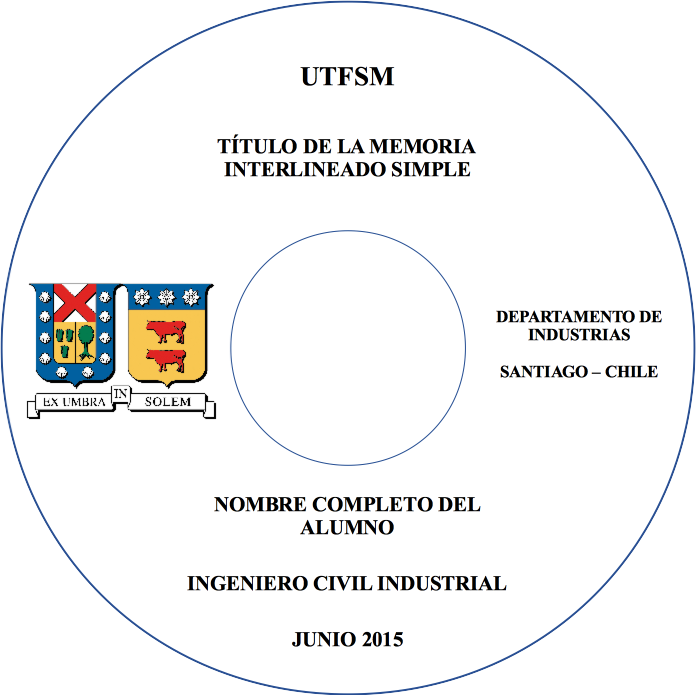
\includegraphics[width=.4\textwidth]{figures/thesis_cd.png}
\caption{Disco Compacto para Memoria UTFSM}
\label{fig:thesis_cd}
\end{figure}


Los CD se guardarán, en la biblioteca, en una caja de acrílico que tendrá una carátula de identificación dividida en tres franjas iguales, con las siguientes leyendas:
\begin{itemize}
		\item
    El escudo a color de la Institución de 20 mm de alto, centrado en la franja superior.
		\item
    El nombre completo del alumno, y centrado dos espacios más abajo el título de la memoria, en la franja del medio
		\item
    El nombre de la Unidad Académica, y renglón más abajo, año. En la franja inferior.
\end{itemize}


\begin{figure}[ht!]
\centering

\includegraphics[width=.4\textwidth]{figures/thesis_cd_cover.png}
\caption{Cubierta de Disco Compacto para Memorias y Tesis UTFSM.}
\label{fig:thesis_cd_cover}
\end{figure}


La carpeta \inlinecode{figures} incluye los diagramas (formato LibreOffice) para modificación e impresión.

%%%%%
\section{Documentos que se incluyen}

Se incluyen (en la carpeta \inlinecode{figures}) logotipos oficiales\footnote{Éstas son imágenes registradas y propiedad intelectual de la UTFSM y del Departamento de Industrias, y no están incluidas en la licencia de esta plantilla. La imagen corporativa de la UTFSM y del Departamento de Industrias están protegidas por leyes chilenas e internacionales de Derechos de autor. Su uso sólo está autorizado a estudiantes y memoristas de la UTFSM para fines de preparación de documentos académicos, incluidas memorias y tesis.}
de la UTFSM y del Departamento de Industrias.

\begin{figure}[ht!]
\centering

\includegraphics[scale = .5]{figures/logousm.png}
\caption{Logotipo de la UTFSM}
\label{fig:logousm}
\end{figure}

\begin{figure}[ht!]
\centering

\includegraphics[scale = .45]{figures/logousmleyenda.png}
\caption{Logotipo de la UTFSM (con leyenda)}
\label{fig:logousmleyenda}
\end{figure}


\begin{figure}[ht!]
\centering

\includegraphics[scale = .75]{figures/logousmind.jpg}
\caption{Logotipo de la UTFSM - Departamento de Industrias}
\label{fig:logousmind}
\end{figure}

\begin{figure}[ht!]
    \centering
    %\rule{4cm}{3cm}
    
\includegraphics[width=.8\textwidth]{figures/logo_utfsm_di.png}
    \caption{Logotipo del Departamento de Industrias, UTFSM (Formato lateral).}
    \label{fig:logodiutfsm}
\end{figure}

\begin{figure}[ht!]
\centering
%\rule{4cm}{3cm}

\includegraphics[width=.3\textwidth]{figures/logoind.png}
\caption{Logotipo del Departamento de Industrias, UTFSM }
\label{fig:logoind1}
\end{figure}


%!TEX root = ../memoria.tex

\chapter{\LaTeX}


\section{Obtener \LaTeX{}}

\LaTeX{} es un sistema de preparación de documentos de alta calidad
visual \citep{latex:whatis}. Si no ha ocupado \LaTeX{} anteriormente,
visite esta página:
\begin{itemize}
\item \href{http://www.latex-project.org/}{http://www.latex-project.org/}
\end{itemize}
\begin{figure}[H]
\begin{centering}
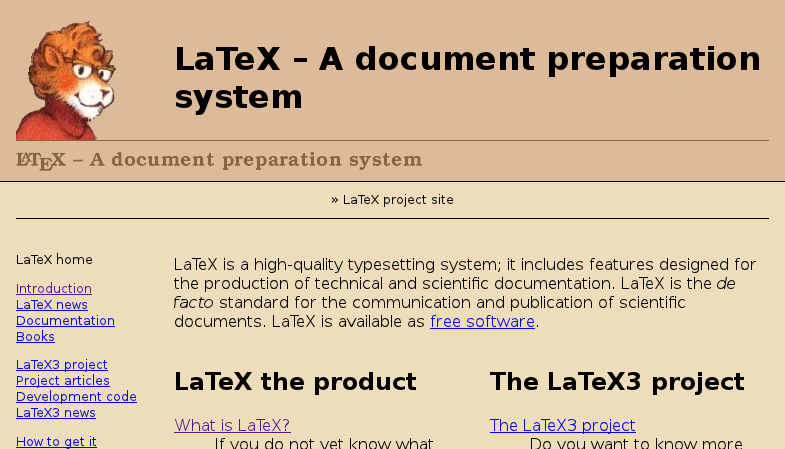
\includegraphics[width=0.7\textwidth]{figures/fig_latex_project_org}
\par\end{centering}

\caption{LaTeX Project}
\end{figure}


Puede obtener, en forma gratuita, las distribuciones de \LaTeX{},
según su plataforma, en:

\begin{description}
\item [Windows] \href{http://miktex.org/}{http://miktex.org/}; también puede
ocupar \href{http://www.tug.org/protext/}{http://www.tug.org/protext/}.

MikTex ofrece una versión básica. Después de instalarlo, asegúrese de descargar los paquetes adicionales requeridos para compilar esta plantilla.

\item [MacOS] \href{http://www.tug.org/mactex/}{http://www.tug.org/mactex/}.

La versión de MacTex es completa e incluye por defecto todos los paquetes necesarios para compilar esta plantilla.

\item [Unix/Linux] \href{http://www.tug.org/texlive/}{http://www.tug.org/texlive/}.

La instalación de TexLive en plataformas *nix es muy sencilla y directa a través de una consola (con permisos de administración):

(K/X)Ubuntu / Debian: \inlinecode{# apt-get install texlive}

Fedora: \inlinecode{# dnf install texlive}

RedHat / CentOS: \inlinecode{# yum install texlive}
\end{description}

Para una referencia completa sobre \LaTeX{}, recomendamos el libro
de \citealp{Lamport94}; aunque para solucionar problemas específicos,
su mejor aliado es Internet. Otros libros que puede consultar se presentan
en la Bibliografía \citep{Mittelbach04,Oetiker06,Roberts05,Borbon2014}.


\section{Editores para \LaTeX}
Existen muchos editores de \LaTeX, la mayoría de ellos de distribución gratuita y con versiones para los distintos sistemas operativos:
\begin{description}
    \item [TexStudio] Mac, Windows y Linux. \href{www.texstudio.org}{www.texstudio.org}.
    \item [TexMaker] Mac, Windows y Linux.  \href{www.xm1math.net/texmaker/}{www.xm1math.net/texmaker/}.
    \item[TeXworks] Mac, Window y Linux. \href{https://www.tug.org/texworks/}{https://www.tug.org/texworks/}
    \item [TexShop] Mac. \href{http://pages.uoregon.edu/koch/texshop/}{http://pages.uoregon.edu/koch/texshop/}.
    \item[Kile] Linux y Mac (vía macports). \href{http://kile.sourceforge.net/}{http://kile.sourceforge.net/}.
    \item[LaTeXila] Linux y Mac (vía Homebrew). \href{https://wiki.gnome.org/Apps/LaTeXila\#Installation}{https://wiki.gnome.org/Apps/LaTeXila\#Installation}.
\end{description}

%...              % Agregar aquí más capítulos
\end{Verbatim}

\section{Para tomar en cuenta (Recomendaciones)}

\subsection{Impresión por ambos lados.}
Este documento está preparado para ser impreso por ambos lados de una hoja (\emph{``twoside''}). Para cambiar esto, en la ``clase de documento'', reemplazar la palabra \emph{``twoside''} por \emph{``oneside''}. Es por esto que encontrará algunas hojas que están en blanco, aparentemente sin motivo.


\begin{Verbatim}[frame=lines, label=\inlinecode{memoria.tex} (extracto)
, fontsize=\footnotesize
, baselinestretch=1
, formatcom=\color{gray}]
%---------------------------------------------------------------------------
%%% DOCUMENT CLASS
\documentclass[
    11pt,
    letterpaper,
    twoside
]{thesis_utfsm}
%---------------------------------------------------------------------------
\end{Verbatim}


Es posible que debas cambiar otras configuraciones también para imprimir por un sólo lado. En particular aquellas páginas en blanco después de los agradecimientos y dedicatoria.

\section{Codificación de caracteres.}

Todos los archivos \inlinecode{*.tex} de esta plantilla han sido preparados ocupando la codificación de caracteres por defecto \emph{unicode} (UTF-8). Windows (y algunas versiones de OSX) ocupan otro tipo de codificación (ej. \emph{Windows-1252} o \emph{Mac Roman}).

Si deseas ocupar esta plantilla y encuentras problemas con los caracteres acentuados, entonces puedes optar por una de estas tres alternativas:
\begin{enumerate}[(i)]
    \item cambiar tu editor (TexMaker, TexStudio, TexShop, etc.) para que ocupe UTF-8 como codificación de caracteres por defecto; o
    \item cambiar la codificación de cada documento \inlinecode{*.tex} para que ocupe la codificación nativa de tu sistema operativo; y, modifica la configuración (\inlinecode{config.tex}) dice:
    
    \inlinecode{\\usepackage[utf8x]\{inputenc\}}, por el texto \inlinecode{\\usepackage[latin1]\{inputenc\}}.
    \item escribir todo ocupando caracteres pre-acentuados (ej. \inlinecode{\\'a} en lugar de á).
\end{enumerate}

\vspace{10mm}
\begin{framed}
    \textbf{Recuerda:} Mezclar documentos de distintas codificaciones puede generarte muchos problemas al momento de compilar.  
\end{framed}


\section{Requisitos}
Los paquetes que se ocupan y son indispensables para la generación este documento están contenidos en el documento de clase \inlinecode{thesis_utfsm.cls}.

Para que funcione correctamente se requiere tener instaladas (como mínimo) las siguientes extensiones \LaTeX{}:
\begin{Verbatim}[frame=lines, label=Paquetes requeridos por \inlinecode{thesis_utfsm.sty}
				, fontsize=\footnotesize
				, baselinestretch=1
				, formatcom=\color{gray}]
geometry    % Márgenes y tamaño de páginas
natbib      % Bibliografía
fontenc     % Codificación de Caracteres
inputenc    % Métodos de entrada (acentos)
fancyhdr    % Encabezados 'Fancy'
chngcntr    % Formatos de Pie de Página
booktabs    % Tablas
tabularx    % Tablas
multirow    % Tablas con multi-columnas / multi-filas
array       % Matrices
float       % Imágenes Flotantes
textcomp    % Símbolos de uso común
endnotes    % Notas finales del documento
paralist    % Mejores Listados
listings    % Mejores Listados
framed      % Marcos
fancybox    % Marcos 'Fancy'
verbatim    % Código Fuente
fancyvrb    % Código Fuente 'Fancy'
wrapfig     % Figuras flotantes
xcolor      % Colores personalizados
graphix     % Mejor inclusión de figuras
subfig      % Figuras con múltiples leyendas
tikz        % Diagramas vectoriales
caption     % Mejores leyendas para figuras y tablas
tocbibind   % Bibliografía en la Tabla de Contenidos
rotating    % Rotación de Tablas
asmmath     % Notación ciéntifica / matemática
asmsymb     % Símbolos matemáticos y letras griegas
txfonts     % Times New Roman (para sistemas distintos de Windows)
microtype   % Mejoras subliminales en el uso de fuentes
parskip     % Separación entre párrafos
\end{Verbatim}

La mayoría de las distribuciones \LaTeX{} traen estos paquetes por defecto, sin embargo, en Windows es posible que deba instalar algunos de ellos si ha instalado el archivo básico de MikTeX.



%%%%%
\section{Diagramación}
Este documento fue realizado usando \LaTeX{} (\citeauthor{latex:whatis}), aunque puede fácilmente ser exportado a LyX (\citeauthor{lyx}). Para ver como transformarlo a Lyx, puede revisar el Wiki (\citeauthor{wikilyx}).

Usted necesitará un compilador de \LaTeX. Los más comúnmente ocupados son \citeauthor{miktex} (Windows) y \citeauthor{mactex} (Apple); Sistemas *nix (incluyendo linux) traen \TeX{} por defecto.

Para una referencia completa sobre \LaTeX{}, recomendamos el libro de \cite{Lamport94}; aunque para solucionar problemas específicos, su mejor aliado es Internet.

% Other Author (Included only in Bibliography)
También puede revisar \citet{Roberts05}, \citet{Oetiker06}, y \citet{Mittelbach04}.

\subsection{Figuras}
La siguiente es una figura basada en el archivo \inlinecode{figures/logoind.png}. En este caso, la descripción de la figura va en la parte inferior (ver \autoref{fig:logoind2}).

% Inclusión de Figuras
\begin{figure}[ht!]
\centering

\includegraphics[width=.4\textwidth]{figures/logoind.png}
\caption[Logotipo Departamento de Industrias]{Logotipo Departamento de Industrias\\
{\scriptsize (Fuente: Departamento de Industrias)}}
\label{fig:logoind2}
\end{figure}

La forma de incorporar la \autoref{fig:logoind2} se muestra a continuación:


\begin{Verbatim}[frame=lines, label=Incorporar \autoref{fig:logoind2}
				, fontsize=\footnotesize, numbers=left
				, baselinestretch=1
				, formatcom=\color{gray}]
\begin{figure}[h]
\centering

\includegraphics[width=.4\textwidth]{figures/logoind.png}
\caption[Logotipo Departamento de Industrias]{Logotipo Departamento de Industrias\\
{\scriptsize (Fuente: Departamento de Industrias)}}
\label{fig:logoind2}
\end{figure}
\end{Verbatim}

Otra forma de incorporar figuras es mediante un \inlinecode{float}. En este caso, la figura es incorporada como una imagen ``flotante'' a un costado del texto  (ver Figura \autoref{fig:logousm_float}).

\begin{wrapfigure}{o}{.4\textwidth}
    \vspace{-20pt}
    \begin{spacing}{1}
        \begin{center}
            
\includegraphics[width=.35\columnwidth]{figures/logousm.png}
            \vspace{-10pt}
            \caption{Logotipo USM (Float)}
            \label{fig:logousm_float}
        \end{center}
    \end{spacing}
    \vspace{-10pt}
\end{wrapfigure}

Lorem ipsum dolor sit amet, consectetuer adipiscing elit. Ut purus elit, vestibulum ut, placerat ac, adipiscing vitae, felis. Curabitur dictum gravida mauris. Nam arcu libero, nonummy eget, consectetuer id, vulputate a, magna. Donec vehicula augue eu neque. Pellentesque habitant morbi tristique senectus et netus et malesuada fames ac turpis egestas. Mauris ut leo. Cras viverra metus rhoncus sem. Nulla et lectus vestibulum urna fringilla ultrices. Phasellus eu tellus sit amet tortor gravida placerat. Integer sapien est, iaculis in, pretium quis, viverra ac, nunc. Praesent eget sem vel leo ultrices bibendum. Aenean faucibus. Morbi dolor nulla, malesuada eu, pulvinar at, mollis ac, nulla. Curabitur auctor semper nulla. Donec varius orci eget risus. Duis nibh mi, congue eu, accumsan eleifend, sagittis quis, diam. Duis eget orci sit amet orci dignissim rutrum.



\begin{Verbatim}[frame=lines, label=\autoref{fig:logousm_float}
				, fontsize=\footnotesize, numbers=left
				, baselinestretch=1
				, formatcom=\color{gray}]
\begin{wrapfigure}{o}{.4\textwidth}
    \vspace{-20pt}
    \begin{spacing}{1}
        \begin{center}
            
\includegraphics[width=.35\columnwidth]{figures/logousm.png}
            \vspace{-10pt}
            \caption{Logotipo USM (Float)}
            \label{fig:logousm_float}
        \end{center}
    \end{spacing}
    \vspace{-10pt}
\end{wrapfigure}
\end{Verbatim}


\subsection{Tablas}

La siguiente es una tabla o cuadro básica (ver \autoref{tbl:temperaturas}). Notar las referencias cruzadas y el título de la tabla en la parte superior.

\begin{table}[h!]
    \caption{Tabla de Temperaturas}\label{tbl:temperaturas}
    \begin{tabularx}{\linewidth}{  l  c  c  X }
    \hline
    \textbf{\textsc{Day}} &  \textbf{\textsc{Min Temp}} 
    		& \textbf{\textsc{Max Temp}} & \textbf{\textsc{Summary}}\\
	  \hline\hline
    Monday & 11C & 22C & A clear day with lots of sunshine.
    However, the strong breeze will bring down the temperatures. \\ \hline
    Tuesday & 9C & 19C & Cloudy with rain, across many northern regions. Clear spells
    across most of Scotland and Northern Ireland,
    but rain reaching the far northwest. \\ \hline
    Wednesday & 10C & 21C & Rain will still linger for the morning.
    Conditions will improve by early afternoon and continue
    throughout the evening. \\
    \hline
    \end{tabularx}
\end{table}

\begin{Verbatim}[frame=lines, label=\autoref{fig:logousm_float}
				, fontsize=\footnotesize, numbers=left
				, baselinestretch=1
				, formatcom=\color{gray}]
\begin{table}[h!]
    \caption{Tabla de Temperaturas}\label{tbl:temperaturas}
    \begin{tabularx}{\linewidth}{  l  c  c  X }
    \hline
    \textbf{\textsc{Day}} &  \textbf{\textsc{Min Temp}} 
    		& \textbf{\textsc{Max Temp}} & \textbf{\textsc{Summary}}\\
	  \hline\hline
    Monday & 11C & 22C & A clear day with lots of sunshine.
    However, the strong breeze will bring down the temperatures. \\ \hline
    Tuesday & 9C & 19C & Cloudy with rain, across many northern regions. Clear spells
    across most of Scotland and Northern Ireland,
    but rain reaching the far northwest. \\ \hline
    Wednesday & 10C & 21C & Rain will still linger for the morning.
    Conditions will improve by early afternoon and continue
    throughout the evening. \\
    \hline
    \end{tabularx}
\end{table}
\end{Verbatim}



\subsubsection{Rotación de Tablas}
En caso de tener tablas muy grandes, o si necesita una tabla rotada.
\begin{sidewaystable}
    \centering
    \caption{Rotación de Tablas}
    \begin{tabularx}{\columnwidth}{X X}
        \hline\hline
        \textbf{Column 1} & \textbf{Column 2}\\
        \hline
        Second First & Second Second\\
        \blindtext & \blindtext\\
        \hline\hline
    \end{tabularx}
\end{sidewaystable}


\newpage

\subsection{Opciones Avanzadas para Gráficos}

Los packetes Ti\emph{k}Z y PGF ofrecen alternativas para la creación de gráficos con las más diversas formas y opciones. Para ver opciones consultar \href{http://www.texample.net/tikz/}{www.texample.net/tikz/}.


\newcommand{\MonetaryLevel}{Monetary level}
\newcommand{\RealLevel}{Real level}
\newcommand{\Firms}{Firms}
\newcommand{\Households}{Households}
\newcommand{\Banks}{Banks}
\newcommand{\Commodities}{Commodities}
\newcommand{\LaborPower}{Labor power}
\newcommand{\Wages}{Wages}
\newcommand{\Consumption}{Consumption}
\newcommand{\Credits}{Credits}
\newcommand{\Withdrawals}{Withdrawals}
\newcommand{\Deposits}{Deposits}
\newcommand{\Repayments}{Repayments}

\newcommand{\yslant}{0.5}
\newcommand{\xslant}{-0.6}

\begin{figure}[H]
\centering
\begin{tikzpicture}[scale=1,every node/.style={minimum size=1cm},on grid]

	% Real level
	\begin{scope}[
		yshift=-120,
		every node/.append style={yslant=\yslant,xslant=\xslant},
		yslant=\yslant,xslant=\xslant
	] 
		% The frame:
		\draw[black, dashed, thin] (0,0) rectangle (7,7); 
		% Agents:
		\draw[fill=red]  
			(5,2) circle (.1) % Firms
			(2,2) circle (.1); % Households
		% Flows:
		\draw[-latex,thin] 
			(2,1.8) to[out=-90,in=-90] (5,1.8); % Labour Powers
		\draw[-latex,thin]
			(5,2.2) to[out=90,in=90] (2,2.2); % Wages
		 % Labels:
		\fill[black]
			(0.5,6.5) node[right, scale=.7] {\RealLevel}	
			(5.1,1.9) node[right,scale=.7]{\textbf{\Firms}}
			(1.9,1.9) node[left,scale=.7]{\textbf{\Households}}
			(2.2,3) node [scale=.6, rotate=40] {\Commodities} 
			(4.8,1) node [scale=.6, rotate=40] {\LaborPower};	
	\end{scope}
	
	% 2 vertical lines for linking agents on the 2 levels
	\draw[ultra thin](3.8,4) to (3.8,-0.32);
	\draw[ultra thin](.8,2.4) to (.8,-1.8);
	
	% Monetary level
	\begin{scope}[
		yshift=0,
		every node/.append style={yslant=\yslant,xslant=\xslant},
		yslant=\yslant,xslant=\xslant
	]
		% The frame:
		\fill[white,fill opacity=.75] (0,0) rectangle (7,7); % Opacity
		\draw[black, dashed, thin] (0,0) rectangle (7,7); 
		 % Agents:
		\draw [fill=red]
			(5,2) circle (.1) % Firms
			(2,2) circle (.1) % Households
			(3.5,5) circle (.1); % Banks
		 % Monetary Flows:
		\draw[-latex, thin]
			(3.65,5.1) to[out=30,in=30] (5.15,2.1); % Credits
		\draw[-latex, thin]
			(5,1.8) to[out=-90,in=-90] (2,1.8); % Wages
		\draw[-latex, thin]
			(1.9,2.1) to[out=150,in=150] (3.4,5.1);  % Deposits
		\draw[-latex, thin]
			(3.6,4.9) to[out=-30,in=-30] (2.1,1.9); % Withdrawals
		\draw[-latex, thin]
			(2,2.2) to[out=90,in=90] (5,2.2); % Consumption
		\draw[-latex, thin]
			(4.85,1.9) to[out=210,in=210] (3.35,4.9) ; % Repayments
		 % Labels:
		\fill[black]
			(0.5,6.5) node[right, scale=.7] {\MonetaryLevel}
			(5.1,1.9) node[right,scale=.7]{\textbf {\Firms}}
			(1.9,1.9) node[left,scale=.7]{\textbf {\Households}}
			(3.5,5.1) node[above,scale=.7]{\textbf {\Banks}}
			(5.5,2.8) node [above, scale=.6, rotate=-100] {\Credits}
			(2.6,1.3) node [above, scale=.6, rotate=-10] {\Withdrawals}
			(2.9,4.25) node [above, scale=.6, rotate=50] {\Repayments}
			(2.6,5) node [above, scale=.6, rotate=25] {\Deposits}
			(4.7,2.9) node [above, scale=.6, rotate=-60] {\Consumption}
			(2.3,1.3) node [below, scale=.6, rotate=-40] {\Wages}; 
	\end{scope} 
\end{tikzpicture}
\caption[Gráficos Avanzados con Tikz]{Gráficos Avanzados con Tikz\\ {\scriptsize (Fuente: \url{www.texample.net})}}
\label{fig:tikz}
\end{figure}


\begin{figure}[ht!]
\centering
\usetikzlibrary{chains,fit,shapes}
\begin{tikzpicture}
\tikzstyle{every path}=[very thick]

\edef\sizetape{0.7cm}
\tikzstyle{tmtape}=[draw,minimum size=\sizetape]
\tikzstyle{tmhead}=[arrow box,draw,minimum size=.5cm,arrow box
arrows={east:.25cm, west:0.25cm}]

%% Draw TM tape
\begin{scope}[start chain=1 going right,node distance=-0.15mm]
    \node [on chain=1,tmtape,draw=none] {$\ldots$};
    \node [on chain=1,tmtape] {};
    \node [on chain=1,tmtape] (input) {b};
    \node [on chain=1,tmtape] {b};
    \node [on chain=1,tmtape] {a};
    \node [on chain=1,tmtape] {a};
    \node [on chain=1,tmtape] {a};
    \node [on chain=1,tmtape] {a};
    \node [on chain=1,tmtape] {};
    \node [on chain=1,tmtape,draw=none] {$\ldots$};
    \node [on chain=1] {\textbf{Input/Output Tape}};
\end{scope}

%% Draw TM Finite Control
\begin{scope}
[shift={(3cm,-5cm)},start chain=circle placed {at=(-\tikzchaincount*60:1.5)}]
\foreach \i in {q_0,q_1,q_2,q_3,\ddots,q_n}
	\node [on chain] {$\i$};

% Arrow to current state
\node (center) {};
\draw[->] (center) -- (circle-2);

\node[rounded corners,draw=black,thick,fit=(circle-1) (circle-2) (circle-3) 
      (circle-4) (circle-5) (circle-6),
			label=below:\textbf{Finite Control}] (fsbox)
		{};
\end{scope}

%% Draw TM head below (input) tape cell
\node [tmhead,yshift=-.3cm] at (input.south) (head) {$q_1$};

%% Link Finite Control with Head
\path[->,draw] (fsbox.north) .. controls (4.5,-1) and (0,-2) .. node[right] 
			(headlinetext)
 			{} 
			(head.south);
\node[xshift=3cm] at (headlinetext)  
			{\begin{tabular}{c} 
				\textbf{Reading and Writing Head} \\  
				\textbf{(moves in both directions)} 
			 \end{tabular}};

\end{tikzpicture}
\caption [Diagrama de la Máquina de Türing]{Diagrama de la Máquina de Türing\\ {\scriptsize (Fuente: \url{www.texample.net})}}
\end{figure}


\begin{figure}[ht!]
\centering
% Styles
\tikzstyle{load}   = [ultra thick,-latex]
\tikzstyle{stress} = [-latex]
\tikzstyle{dim}    = [latex-latex]
\tikzstyle{axis}   = [-latex,black!55]

% Drawing Views
\tikzstyle{isometric}=[x={(0.710cm,-0.410cm)},y={(0cm,0.820cm)},z={(-0.710cm,-0.410cm)}]
\tikzstyle{dimetric} =[x={(0.935cm,-0.118cm)},y={(0cm,0.943cm)},z={(-0.354cm,-0.312cm)}]
\tikzstyle{dimetric2}=[x={(0.935cm,-0.118cm)},z={(0cm,0.943cm)},y={(+0.354cm,+0.312cm)}]
\tikzstyle{trimetric}=[x={(0.926cm,-0.207cm)},y={(0cm,0.837cm)},z={(-0.378cm,-0.507cm)}]

  \begin{tikzpicture}[scale=.8]
    \node (origin) at (0,0) {}; % shift relative baseline
    \coordinate (O) at (2,3);
    \draw[fill=gray!10] (O) circle (1);
    \draw[fill=white] (O) circle (0.75) node[below,yshift=-1.125cm] {Signpost Cross Section};
    \draw[dim] (O) ++(-0.75,0) -- ++(1.5,0) node[midway,above] {$d_i$};
    \draw[dim] (O) ++(-1,1.25) -- ++(2,0) node[midway,above] {$d_o$}; 
    \foreach \x in {-1,1} {
      \draw (O) ++(\x,0.25) -- ++(0,1.25);
    }
  \end{tikzpicture}%
  \begin{tikzpicture}[dimetric2]
        \coordinate (O) at (0,0,0);
        \draw[axis] (O) -- ++(6,0,0) node[right] {$x$};
        \draw[axis] (O) -- ++(0,6,0) node[above right] {$y$};
        \draw[axis] (O) -- ++(0,0,6) node[above] {$z$};
        \draw[fill=gray!50] (0,0,-0.5) circle (0.5); 
        \fill[fill=gray!50] (-0.46,-0.2,-0.5) -- (0.46,0.2,-0.5) -- (0.46,0.2,0) -- (-0.46,-0.2,0) -- cycle;
        \draw[fill=gray!20] (O) circle (0.5);
    \draw (0.46,0.2,-0.5) -- ++(0,0,0.5) node[below right,pos=0.0] {Fixed Support};
    \draw (-0.46,-0.2,-0.5) -- ++(0,0,0.5);
    \draw[fill=gray!10] (O) circle (0.2);
    \fill[fill=gray!10] (-0.175,-0.1,0) -- (0.175,0.1,0) -- ++(0,0,4) -- (-0.175,-0.1,4) -- cycle;
    \draw (-0.175,-0.1,0) -- ++(0,0,4);
    \draw (0.175,0.1,0) -- ++(0,0,4) node[right,midway] {Steel Post};
    \draw (4,0,3.95) -- ++(0,0,-1);
    \foreach \z in {0.5,0.75,...,5} {
      \draw[-latex] (-2*\z/5-0.2,0,\z) -- (-0.2,0,\z);
    }
    \draw[load] (0,0,4) -- ++(0,0,-1.25) node[right,xshift=0.1cm] {$F_{z1}$};
    \draw[fill=gray!20] (-0.25,-0.25,5) -- (4,-0.25,5) -- (4,+0.25,5) -- (-0.25,+0.25,5) -- cycle; 
    \draw[fill=gray!50] (+4.00,-0.25,4) -- (4,+0.25,4) -- (4,+0.25,5) -- (+4.00,-0.25,5) -- cycle; 
    \draw[fill=gray!10] (-0.25,-0.25,4) -- (4,-0.25,4) -- (4,-0.25,5) -- (-0.25,-0.25,5) -- cycle; 
    \draw (4.05,0,4) -- ++(1,0,0);
    \draw (4.05,0,5) -- ++(1,0,0);
    \draw[dim] (4.5,0,0) -- ++(0,0,4) node[midway,right] {$h_1$};
    \draw[dim] (4.5,0,4) -- ++(0,0,1) node[midway,right] {$h_2$};
    \draw[dim] (0,0,3.4) -- ++(4,0,0) node[midway,below] {$b_2$};
    \coordinate (P) at (2,-0.25,4.5);
    \draw (P) -- ++(0,0,0.25);
    \draw (P) -- ++(0.25,0,0);
    \draw[dim] (2.125,-0.25,4.5) -- ++(0,0,-0.5) node[midway,right] {$z_1$};
    \draw[dim] (2,-0.25,4.625) -- ++(-2,0,0) node[midway,below] {$x_1$};
    \draw[load] (2,-2.45,4.5) -- ++(0,2.2,0) node[pos=0.0,right,xshift=0.08cm] {$F_{y1}$};
    \draw[axis,dashed,-] (O) -- (0,0,5);
    \draw (0,0,5.5) -- ++(4,0,0) node[midway,above] {$w_{z}$};
    \foreach \x in {0,0.25,...,4} {
      \draw[-latex] (\x,0,5.5) -- ++(0,0,-0.5);
    }
    \draw (-0.2,0,0) -- ++(-2,0,5) node[above,xshift=0.5cm] {$w_{x}=\frac{z}{h_1+h_2} w_0$};
  \end{tikzpicture} 
  \caption [Cargas aplicadas sobre un poste.]{Cargas aplicadas sobre un poste.\\ {\scriptsize (Fuente: \url{www.texample.net})}}
\end{figure}




%!TEX root = ../memoria.tex

\chapter{Formatos UTFSM para Memorias y Tesis de Grado }

Los formatos exigidos (y ocupados en este documento) por el Departamento de Industrias y la UTFSM incluyen:

\begin{description}
\item[Tipografía.] Fuente \emph{Times New Roman} o similar de 11 o 12 puntos (pts.), con interlineado de 1 espacio (máximo 1,5 espacios).
\item[Márgenes.] Margen izquierdo (o interno) de $3.5cm$ (mínimo). Margen derecho (o externo) de $2cm$ (mínimo). Note que esto cambia para páginas pares e impares para facilitar el empaste de documentos impresos por ambos lados de cada hoja.
\item[Citas bibliogáficas.] Las citas bibliográficas se harán siguiendo normas de la UTFSM (éstas están basadas en las normas \emph{APA} (usada en este documento), \emph{AMS}, o \emph{IEEE}). Ejemplo:

\begin{quote}
    ``\LaTeX{} es un sistema de diagramación de documentos.'' \citep{Lamport94}.
\end{quote}

Este documento ocupa estas normas. Revisar la bibliografía que se adjunta para ver un ejemplo.

\item[Numeración de Títulos.] El texto del informe final debe ser subdivido en: capítulos y sub-capítulos. La numeración de capítulos estará basada en esquema con división de puntos para los sub-capítulos, es decir: Capítulo 1, Sub-capítulo 1.1, etc.
\item[Numeración de Páginas.] Todas las páginas (con excepción de la portada) deben estar numeradas. El preámbulo (Índices, Resumen, Abstract, etc.) debe llevar numeración distinta del desarrollo (capítulos) del documento.
\item[Numeración de Formulas, Tablas y Figuras.] Las fórmulas, figuras y tablas correspondientes a un mismo capítulo, se identificarán mediante dos números. El primero corresponde al capítulo pertinente y el segundo al número de orden correlativo.


Los números con que se identifican las fórmulas se colocarán al extremo derecho de las mismas y entre paréntesis. Ejemplo (\autoref{eq:eq_example}):
\begin{equation}
f(x) = x^2-2x+1
\label{eq:eq_example}
\end{equation}

Las ilustraciones (gráficos, láminas, fotografías, etc.) en lo posible deben quedar ubicadas dentro de la página que se les referencia. Los números correspondientes a figuras se colocarán en la parte inferior de las mismas, seguidos de título o breve explicación de la figura. Ver \autoref{fig:figure_example}.
	\begin{figure}[ht!]
	\centering
	%\rule{4cm}{3cm}
	
\includegraphics[width=.3\textwidth]{figures/logoind.png}
	
	\caption[Logotipo del Departamento de Industrias, UTFSM.]{Logotipo del Departamento de Industrias, UTFSM.\\
	{\footnotesize (Fuente: Departamento de Industrias, 2016.)}}
	
	\label{fig:figure_example}
	\end{figure}

Los números asignados a las tablas se colocarán en la parte superior de ellas, seguidos de los títulos correspondientes. Ver \autoref{tbl:table_example}

\begin{table}[ht]
\centering
\caption{Ejemplo de Numeración de Tablas.}
\begin{tabular}{p{3cm}|p{3cm}|p{3cm}}
\hline
\textbf{Columna 1} & \textbf{Columna 2} & \textbf{Columna 3} \\
\hline\hline
... & ... & ... \\
\hline
... & ... & ... \\
\hline
\end{tabular}
\label{tbl:table_example}
\end{table}

\end{description}

\section{Otros Formatos UTFSM}
\subsection{Formato de las Cubiertas (Empaste)}

La cubierta o tapa será de empaste duro, cubierta de vinilo o similar de color NEGRO con letras doradas, según se muestran en \autoref{fig:thesis_cover} y \autoref{fig:thesis_cover_lateral}.
\begin{figure}[ht!]
\centering

\includegraphics[width=.7\textwidth]{figures/thesis_cover.png}
\caption{Cubierta (Empaste) Memorias y Tesis UTFSM.}
\label{fig:thesis_cover}
\end{figure}

\begin{figure}[ht!]
\centering

\includegraphics[width=.7\textwidth]{figures/thesis_cover_lateral.png}
\caption{Lomo del Empaste para Memorias y Tesis UTFSM.}
\label{fig:thesis_cover_lateral}
\end{figure}

\subsection{Formato del Disco Compacto}

El CD/DVD debe tener una carátula de identificación circular con fondo blanco, conteniendo las siguientes leyendas:

\begin{itemize}
		\item
    Centrado en la parte superior: UTFSM, con letras mayúsculas en negrita tamaño 12. A renglón seguido el nombre de la Unidad Académica con letras mayúsculas en negrita tamaño 10.
		\item
    Centrado en la parte inferior el nombre completo del alumno con letras mayúsculas en negrita tamaño 10.
		\item
    Tres espacios más abajo y centrado, “TÍTULO DE LA MEMORIA”, con letras mayúsculas en negrita tamaño 10.
		\item
    Dos espacios más abajo y centrado MES –AÑO, con letras mayúsculas en negrita tamaño 10.
    En el lado izquierdo y centrado, el escudo en colores de la Institución.
		\item
    En el lado derecho y centrado, NOMBRE DE LA UNIDAD ACADÉMICA y la ubicación CIUDAD – PAIS, con letras mayúsculas en negrita tamaño 8.
\end{itemize}

\begin{figure}[ht!]
\centering
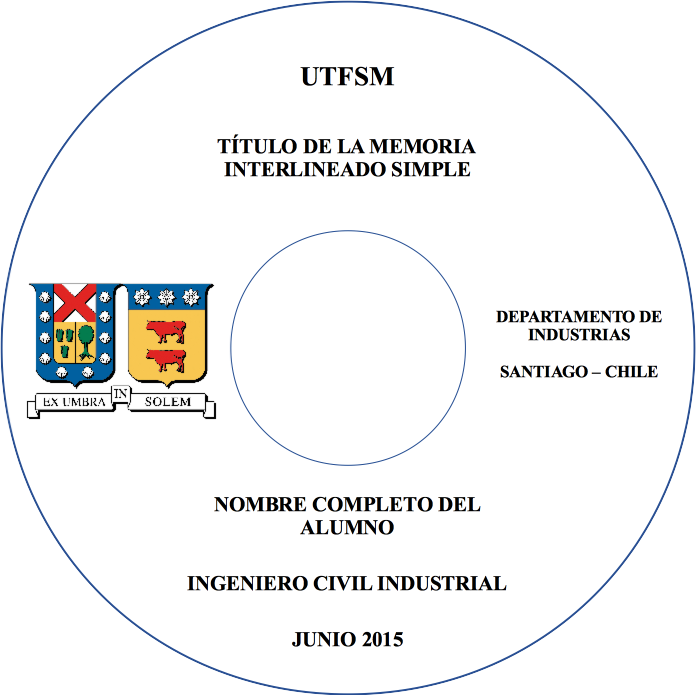
\includegraphics[width=.4\textwidth]{figures/thesis_cd.png}
\caption{Disco Compacto para Memoria UTFSM}
\label{fig:thesis_cd}
\end{figure}


Los CD se guardarán, en la biblioteca, en una caja de acrílico que tendrá una carátula de identificación dividida en tres franjas iguales, con las siguientes leyendas:
\begin{itemize}
		\item
    El escudo a color de la Institución de 20 mm de alto, centrado en la franja superior.
		\item
    El nombre completo del alumno, y centrado dos espacios más abajo el título de la memoria, en la franja del medio
		\item
    El nombre de la Unidad Académica, y renglón más abajo, año. En la franja inferior.
\end{itemize}


\begin{figure}[ht!]
\centering

\includegraphics[width=.4\textwidth]{figures/thesis_cd_cover.png}
\caption{Cubierta de Disco Compacto para Memorias y Tesis UTFSM.}
\label{fig:thesis_cd_cover}
\end{figure}


La carpeta \inlinecode{figures} incluye los diagramas (formato LibreOffice) para modificación e impresión.

%%%%%
\section{Documentos que se incluyen}

Se incluyen (en la carpeta \inlinecode{figures}) logotipos oficiales\footnote{Éstas son imágenes registradas y propiedad intelectual de la UTFSM y del Departamento de Industrias, y no están incluidas en la licencia de esta plantilla. La imagen corporativa de la UTFSM y del Departamento de Industrias están protegidas por leyes chilenas e internacionales de Derechos de autor. Su uso sólo está autorizado a estudiantes y memoristas de la UTFSM para fines de preparación de documentos académicos, incluidas memorias y tesis.}
de la UTFSM y del Departamento de Industrias.

\begin{figure}[ht!]
\centering

\includegraphics[scale = .5]{figures/logousm.png}
\caption{Logotipo de la UTFSM}
\label{fig:logousm}
\end{figure}

\begin{figure}[ht!]
\centering

\includegraphics[scale = .45]{figures/logousmleyenda.png}
\caption{Logotipo de la UTFSM (con leyenda)}
\label{fig:logousmleyenda}
\end{figure}


\begin{figure}[ht!]
\centering

\includegraphics[scale = .75]{figures/logousmind.jpg}
\caption{Logotipo de la UTFSM - Departamento de Industrias}
\label{fig:logousmind}
\end{figure}

\begin{figure}[ht!]
    \centering
    %\rule{4cm}{3cm}
    
\includegraphics[width=.8\textwidth]{figures/logo_utfsm_di.png}
    \caption{Logotipo del Departamento de Industrias, UTFSM (Formato lateral).}
    \label{fig:logodiutfsm}
\end{figure}

\begin{figure}[ht!]
\centering
%\rule{4cm}{3cm}

\includegraphics[width=.3\textwidth]{figures/logoind.png}
\caption{Logotipo del Departamento de Industrias, UTFSM }
\label{fig:logoind1}
\end{figure}


%!TEX root = ../memoria.tex

\chapter{\LaTeX}


\section{Obtener \LaTeX{}}

\LaTeX{} es un sistema de preparación de documentos de alta calidad
visual \citep{latex:whatis}. Si no ha ocupado \LaTeX{} anteriormente,
visite esta página:
\begin{itemize}
\item \href{http://www.latex-project.org/}{http://www.latex-project.org/}
\end{itemize}
\begin{figure}[H]
\begin{centering}
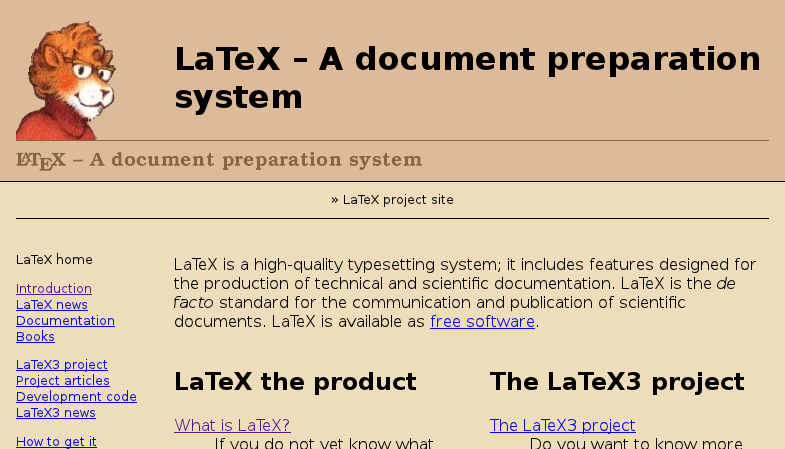
\includegraphics[width=0.7\textwidth]{figures/fig_latex_project_org}
\par\end{centering}

\caption{LaTeX Project}
\end{figure}


Puede obtener, en forma gratuita, las distribuciones de \LaTeX{},
según su plataforma, en:

\begin{description}
\item [Windows] \href{http://miktex.org/}{http://miktex.org/}; también puede
ocupar \href{http://www.tug.org/protext/}{http://www.tug.org/protext/}.

MikTex ofrece una versión básica. Después de instalarlo, asegúrese de descargar los paquetes adicionales requeridos para compilar esta plantilla.

\item [MacOS] \href{http://www.tug.org/mactex/}{http://www.tug.org/mactex/}.

La versión de MacTex es completa e incluye por defecto todos los paquetes necesarios para compilar esta plantilla.

\item [Unix/Linux] \href{http://www.tug.org/texlive/}{http://www.tug.org/texlive/}.

La instalación de TexLive en plataformas *nix es muy sencilla y directa a través de una consola (con permisos de administración):

(K/X)Ubuntu / Debian: \inlinecode{# apt-get install texlive}

Fedora: \inlinecode{# dnf install texlive}

RedHat / CentOS: \inlinecode{# yum install texlive}
\end{description}

Para una referencia completa sobre \LaTeX{}, recomendamos el libro
de \citealp{Lamport94}; aunque para solucionar problemas específicos,
su mejor aliado es Internet. Otros libros que puede consultar se presentan
en la Bibliografía \citep{Mittelbach04,Oetiker06,Roberts05,Borbon2014}.


\section{Editores para \LaTeX}
Existen muchos editores de \LaTeX, la mayoría de ellos de distribución gratuita y con versiones para los distintos sistemas operativos:
\begin{description}
    \item [TexStudio] Mac, Windows y Linux. \href{www.texstudio.org}{www.texstudio.org}.
    \item [TexMaker] Mac, Windows y Linux.  \href{www.xm1math.net/texmaker/}{www.xm1math.net/texmaker/}.
    \item[TeXworks] Mac, Window y Linux. \href{https://www.tug.org/texworks/}{https://www.tug.org/texworks/}
    \item [TexShop] Mac. \href{http://pages.uoregon.edu/koch/texshop/}{http://pages.uoregon.edu/koch/texshop/}.
    \item[Kile] Linux y Mac (vía macports). \href{http://kile.sourceforge.net/}{http://kile.sourceforge.net/}.
    \item[LaTeXila] Linux y Mac (vía Homebrew). \href{https://wiki.gnome.org/Apps/LaTeXila\#Installation}{https://wiki.gnome.org/Apps/LaTeXila\#Installation}.
\end{description}

%...              % Agregar aquí más capítulos
\end{Verbatim}

\section{Para tomar en cuenta (Recomendaciones)}

\subsection{Impresión por ambos lados.}
Este documento está preparado para ser impreso por ambos lados de una hoja (\emph{``twoside''}). Para cambiar esto, en la ``clase de documento'', reemplazar la palabra \emph{``twoside''} por \emph{``oneside''}. Es por esto que encontrará algunas hojas que están en blanco, aparentemente sin motivo.


\begin{Verbatim}[frame=lines, label=\inlinecode{memoria.tex} (extracto)
, fontsize=\footnotesize
, baselinestretch=1
, formatcom=\color{gray}]
%---------------------------------------------------------------------------
%%% DOCUMENT CLASS
\documentclass[
    11pt,
    letterpaper,
    twoside
]{thesis_utfsm}
%---------------------------------------------------------------------------
\end{Verbatim}


Es posible que debas cambiar otras configuraciones también para imprimir por un sólo lado. En particular aquellas páginas en blanco después de los agradecimientos y dedicatoria.

\section{Codificación de caracteres.}

Todos los archivos \inlinecode{*.tex} de esta plantilla han sido preparados ocupando la codificación de caracteres por defecto \emph{unicode} (UTF-8). Windows (y algunas versiones de OSX) ocupan otro tipo de codificación (ej. \emph{Windows-1252} o \emph{Mac Roman}).

Si deseas ocupar esta plantilla y encuentras problemas con los caracteres acentuados, entonces puedes optar por una de estas tres alternativas:
\begin{enumerate}[(i)]
    \item cambiar tu editor (TexMaker, TexStudio, TexShop, etc.) para que ocupe UTF-8 como codificación de caracteres por defecto; o
    \item cambiar la codificación de cada documento \inlinecode{*.tex} para que ocupe la codificación nativa de tu sistema operativo; y, modifica la configuración (\inlinecode{config.tex}) dice:
    
    \inlinecode{\\usepackage[utf8x]\{inputenc\}}, por el texto \inlinecode{\\usepackage[latin1]\{inputenc\}}.
    \item escribir todo ocupando caracteres pre-acentuados (ej. \inlinecode{\\'a} en lugar de á).
\end{enumerate}

\vspace{10mm}
\begin{framed}
    \textbf{Recuerda:} Mezclar documentos de distintas codificaciones puede generarte muchos problemas al momento de compilar.  
\end{framed}


\section{Requisitos}
Los paquetes que se ocupan y son indispensables para la generación este documento están contenidos en el documento de clase \inlinecode{thesis_utfsm.cls}.

Para que funcione correctamente se requiere tener instaladas (como mínimo) las siguientes extensiones \LaTeX{}:
\begin{Verbatim}[frame=lines, label=Paquetes requeridos por \inlinecode{thesis_utfsm.sty}
				, fontsize=\footnotesize
				, baselinestretch=1
				, formatcom=\color{gray}]
geometry    % Márgenes y tamaño de páginas
natbib      % Bibliografía
fontenc     % Codificación de Caracteres
inputenc    % Métodos de entrada (acentos)
fancyhdr    % Encabezados 'Fancy'
chngcntr    % Formatos de Pie de Página
booktabs    % Tablas
tabularx    % Tablas
multirow    % Tablas con multi-columnas / multi-filas
array       % Matrices
float       % Imágenes Flotantes
textcomp    % Símbolos de uso común
endnotes    % Notas finales del documento
paralist    % Mejores Listados
listings    % Mejores Listados
framed      % Marcos
fancybox    % Marcos 'Fancy'
verbatim    % Código Fuente
fancyvrb    % Código Fuente 'Fancy'
wrapfig     % Figuras flotantes
xcolor      % Colores personalizados
graphix     % Mejor inclusión de figuras
subfig      % Figuras con múltiples leyendas
tikz        % Diagramas vectoriales
caption     % Mejores leyendas para figuras y tablas
tocbibind   % Bibliografía en la Tabla de Contenidos
rotating    % Rotación de Tablas
asmmath     % Notación ciéntifica / matemática
asmsymb     % Símbolos matemáticos y letras griegas
txfonts     % Times New Roman (para sistemas distintos de Windows)
microtype   % Mejoras subliminales en el uso de fuentes
parskip     % Separación entre párrafos
\end{Verbatim}

La mayoría de las distribuciones \LaTeX{} traen estos paquetes por defecto, sin embargo, en Windows es posible que deba instalar algunos de ellos si ha instalado el archivo básico de MikTeX.



%%%%%
\section{Diagramación}
Este documento fue realizado usando \LaTeX{} (\citeauthor{latex:whatis}), aunque puede fácilmente ser exportado a LyX (\citeauthor{lyx}). Para ver como transformarlo a Lyx, puede revisar el Wiki (\citeauthor{wikilyx}).

Usted necesitará un compilador de \LaTeX. Los más comúnmente ocupados son \citeauthor{miktex} (Windows) y \citeauthor{mactex} (Apple); Sistemas *nix (incluyendo linux) traen \TeX{} por defecto.

Para una referencia completa sobre \LaTeX{}, recomendamos el libro de \cite{Lamport94}; aunque para solucionar problemas específicos, su mejor aliado es Internet.

% Other Author (Included only in Bibliography)
También puede revisar \citet{Roberts05}, \citet{Oetiker06}, y \citet{Mittelbach04}.

\subsection{Figuras}
La siguiente es una figura basada en el archivo \inlinecode{figures/logoind.png}. En este caso, la descripción de la figura va en la parte inferior (ver \autoref{fig:logoind2}).

% Inclusión de Figuras
\begin{figure}[ht!]
\centering

\includegraphics[width=.4\textwidth]{figures/logoind.png}
\caption[Logotipo Departamento de Industrias]{Logotipo Departamento de Industrias\\
{\scriptsize (Fuente: Departamento de Industrias)}}
\label{fig:logoind2}
\end{figure}

La forma de incorporar la \autoref{fig:logoind2} se muestra a continuación:


\begin{Verbatim}[frame=lines, label=Incorporar \autoref{fig:logoind2}
				, fontsize=\footnotesize, numbers=left
				, baselinestretch=1
				, formatcom=\color{gray}]
\begin{figure}[h]
\centering

\includegraphics[width=.4\textwidth]{figures/logoind.png}
\caption[Logotipo Departamento de Industrias]{Logotipo Departamento de Industrias\\
{\scriptsize (Fuente: Departamento de Industrias)}}
\label{fig:logoind2}
\end{figure}
\end{Verbatim}

Otra forma de incorporar figuras es mediante un \inlinecode{float}. En este caso, la figura es incorporada como una imagen ``flotante'' a un costado del texto  (ver Figura \autoref{fig:logousm_float}).

\begin{wrapfigure}{o}{.4\textwidth}
    \vspace{-20pt}
    \begin{spacing}{1}
        \begin{center}
            
\includegraphics[width=.35\columnwidth]{figures/logousm.png}
            \vspace{-10pt}
            \caption{Logotipo USM (Float)}
            \label{fig:logousm_float}
        \end{center}
    \end{spacing}
    \vspace{-10pt}
\end{wrapfigure}

Lorem ipsum dolor sit amet, consectetuer adipiscing elit. Ut purus elit, vestibulum ut, placerat ac, adipiscing vitae, felis. Curabitur dictum gravida mauris. Nam arcu libero, nonummy eget, consectetuer id, vulputate a, magna. Donec vehicula augue eu neque. Pellentesque habitant morbi tristique senectus et netus et malesuada fames ac turpis egestas. Mauris ut leo. Cras viverra metus rhoncus sem. Nulla et lectus vestibulum urna fringilla ultrices. Phasellus eu tellus sit amet tortor gravida placerat. Integer sapien est, iaculis in, pretium quis, viverra ac, nunc. Praesent eget sem vel leo ultrices bibendum. Aenean faucibus. Morbi dolor nulla, malesuada eu, pulvinar at, mollis ac, nulla. Curabitur auctor semper nulla. Donec varius orci eget risus. Duis nibh mi, congue eu, accumsan eleifend, sagittis quis, diam. Duis eget orci sit amet orci dignissim rutrum.



\begin{Verbatim}[frame=lines, label=\autoref{fig:logousm_float}
				, fontsize=\footnotesize, numbers=left
				, baselinestretch=1
				, formatcom=\color{gray}]
\begin{wrapfigure}{o}{.4\textwidth}
    \vspace{-20pt}
    \begin{spacing}{1}
        \begin{center}
            
\includegraphics[width=.35\columnwidth]{figures/logousm.png}
            \vspace{-10pt}
            \caption{Logotipo USM (Float)}
            \label{fig:logousm_float}
        \end{center}
    \end{spacing}
    \vspace{-10pt}
\end{wrapfigure}
\end{Verbatim}


\subsection{Tablas}

La siguiente es una tabla o cuadro básica (ver \autoref{tbl:temperaturas}). Notar las referencias cruzadas y el título de la tabla en la parte superior.

\begin{table}[h!]
    \caption{Tabla de Temperaturas}\label{tbl:temperaturas}
    \begin{tabularx}{\linewidth}{  l  c  c  X }
    \hline
    \textbf{\textsc{Day}} &  \textbf{\textsc{Min Temp}} 
    		& \textbf{\textsc{Max Temp}} & \textbf{\textsc{Summary}}\\
	  \hline\hline
    Monday & 11C & 22C & A clear day with lots of sunshine.
    However, the strong breeze will bring down the temperatures. \\ \hline
    Tuesday & 9C & 19C & Cloudy with rain, across many northern regions. Clear spells
    across most of Scotland and Northern Ireland,
    but rain reaching the far northwest. \\ \hline
    Wednesday & 10C & 21C & Rain will still linger for the morning.
    Conditions will improve by early afternoon and continue
    throughout the evening. \\
    \hline
    \end{tabularx}
\end{table}

\begin{Verbatim}[frame=lines, label=\autoref{fig:logousm_float}
				, fontsize=\footnotesize, numbers=left
				, baselinestretch=1
				, formatcom=\color{gray}]
\begin{table}[h!]
    \caption{Tabla de Temperaturas}\label{tbl:temperaturas}
    \begin{tabularx}{\linewidth}{  l  c  c  X }
    \hline
    \textbf{\textsc{Day}} &  \textbf{\textsc{Min Temp}} 
    		& \textbf{\textsc{Max Temp}} & \textbf{\textsc{Summary}}\\
	  \hline\hline
    Monday & 11C & 22C & A clear day with lots of sunshine.
    However, the strong breeze will bring down the temperatures. \\ \hline
    Tuesday & 9C & 19C & Cloudy with rain, across many northern regions. Clear spells
    across most of Scotland and Northern Ireland,
    but rain reaching the far northwest. \\ \hline
    Wednesday & 10C & 21C & Rain will still linger for the morning.
    Conditions will improve by early afternoon and continue
    throughout the evening. \\
    \hline
    \end{tabularx}
\end{table}
\end{Verbatim}



\subsubsection{Rotación de Tablas}
En caso de tener tablas muy grandes, o si necesita una tabla rotada.
\begin{sidewaystable}
    \centering
    \caption{Rotación de Tablas}
    \begin{tabularx}{\columnwidth}{X X}
        \hline\hline
        \textbf{Column 1} & \textbf{Column 2}\\
        \hline
        Second First & Second Second\\
        \blindtext & \blindtext\\
        \hline\hline
    \end{tabularx}
\end{sidewaystable}


\newpage

\subsection{Opciones Avanzadas para Gráficos}

Los packetes Ti\emph{k}Z y PGF ofrecen alternativas para la creación de gráficos con las más diversas formas y opciones. Para ver opciones consultar \href{http://www.texample.net/tikz/}{www.texample.net/tikz/}.


\newcommand{\MonetaryLevel}{Monetary level}
\newcommand{\RealLevel}{Real level}
\newcommand{\Firms}{Firms}
\newcommand{\Households}{Households}
\newcommand{\Banks}{Banks}
\newcommand{\Commodities}{Commodities}
\newcommand{\LaborPower}{Labor power}
\newcommand{\Wages}{Wages}
\newcommand{\Consumption}{Consumption}
\newcommand{\Credits}{Credits}
\newcommand{\Withdrawals}{Withdrawals}
\newcommand{\Deposits}{Deposits}
\newcommand{\Repayments}{Repayments}

\newcommand{\yslant}{0.5}
\newcommand{\xslant}{-0.6}

\begin{figure}[H]
\centering
\begin{tikzpicture}[scale=1,every node/.style={minimum size=1cm},on grid]

	% Real level
	\begin{scope}[
		yshift=-120,
		every node/.append style={yslant=\yslant,xslant=\xslant},
		yslant=\yslant,xslant=\xslant
	] 
		% The frame:
		\draw[black, dashed, thin] (0,0) rectangle (7,7); 
		% Agents:
		\draw[fill=red]  
			(5,2) circle (.1) % Firms
			(2,2) circle (.1); % Households
		% Flows:
		\draw[-latex,thin] 
			(2,1.8) to[out=-90,in=-90] (5,1.8); % Labour Powers
		\draw[-latex,thin]
			(5,2.2) to[out=90,in=90] (2,2.2); % Wages
		 % Labels:
		\fill[black]
			(0.5,6.5) node[right, scale=.7] {\RealLevel}	
			(5.1,1.9) node[right,scale=.7]{\textbf{\Firms}}
			(1.9,1.9) node[left,scale=.7]{\textbf{\Households}}
			(2.2,3) node [scale=.6, rotate=40] {\Commodities} 
			(4.8,1) node [scale=.6, rotate=40] {\LaborPower};	
	\end{scope}
	
	% 2 vertical lines for linking agents on the 2 levels
	\draw[ultra thin](3.8,4) to (3.8,-0.32);
	\draw[ultra thin](.8,2.4) to (.8,-1.8);
	
	% Monetary level
	\begin{scope}[
		yshift=0,
		every node/.append style={yslant=\yslant,xslant=\xslant},
		yslant=\yslant,xslant=\xslant
	]
		% The frame:
		\fill[white,fill opacity=.75] (0,0) rectangle (7,7); % Opacity
		\draw[black, dashed, thin] (0,0) rectangle (7,7); 
		 % Agents:
		\draw [fill=red]
			(5,2) circle (.1) % Firms
			(2,2) circle (.1) % Households
			(3.5,5) circle (.1); % Banks
		 % Monetary Flows:
		\draw[-latex, thin]
			(3.65,5.1) to[out=30,in=30] (5.15,2.1); % Credits
		\draw[-latex, thin]
			(5,1.8) to[out=-90,in=-90] (2,1.8); % Wages
		\draw[-latex, thin]
			(1.9,2.1) to[out=150,in=150] (3.4,5.1);  % Deposits
		\draw[-latex, thin]
			(3.6,4.9) to[out=-30,in=-30] (2.1,1.9); % Withdrawals
		\draw[-latex, thin]
			(2,2.2) to[out=90,in=90] (5,2.2); % Consumption
		\draw[-latex, thin]
			(4.85,1.9) to[out=210,in=210] (3.35,4.9) ; % Repayments
		 % Labels:
		\fill[black]
			(0.5,6.5) node[right, scale=.7] {\MonetaryLevel}
			(5.1,1.9) node[right,scale=.7]{\textbf {\Firms}}
			(1.9,1.9) node[left,scale=.7]{\textbf {\Households}}
			(3.5,5.1) node[above,scale=.7]{\textbf {\Banks}}
			(5.5,2.8) node [above, scale=.6, rotate=-100] {\Credits}
			(2.6,1.3) node [above, scale=.6, rotate=-10] {\Withdrawals}
			(2.9,4.25) node [above, scale=.6, rotate=50] {\Repayments}
			(2.6,5) node [above, scale=.6, rotate=25] {\Deposits}
			(4.7,2.9) node [above, scale=.6, rotate=-60] {\Consumption}
			(2.3,1.3) node [below, scale=.6, rotate=-40] {\Wages}; 
	\end{scope} 
\end{tikzpicture}
\caption[Gráficos Avanzados con Tikz]{Gráficos Avanzados con Tikz\\ {\scriptsize (Fuente: \url{www.texample.net})}}
\label{fig:tikz}
\end{figure}


\begin{figure}[ht!]
\centering
\usetikzlibrary{chains,fit,shapes}
\begin{tikzpicture}
\tikzstyle{every path}=[very thick]

\edef\sizetape{0.7cm}
\tikzstyle{tmtape}=[draw,minimum size=\sizetape]
\tikzstyle{tmhead}=[arrow box,draw,minimum size=.5cm,arrow box
arrows={east:.25cm, west:0.25cm}]

%% Draw TM tape
\begin{scope}[start chain=1 going right,node distance=-0.15mm]
    \node [on chain=1,tmtape,draw=none] {$\ldots$};
    \node [on chain=1,tmtape] {};
    \node [on chain=1,tmtape] (input) {b};
    \node [on chain=1,tmtape] {b};
    \node [on chain=1,tmtape] {a};
    \node [on chain=1,tmtape] {a};
    \node [on chain=1,tmtape] {a};
    \node [on chain=1,tmtape] {a};
    \node [on chain=1,tmtape] {};
    \node [on chain=1,tmtape,draw=none] {$\ldots$};
    \node [on chain=1] {\textbf{Input/Output Tape}};
\end{scope}

%% Draw TM Finite Control
\begin{scope}
[shift={(3cm,-5cm)},start chain=circle placed {at=(-\tikzchaincount*60:1.5)}]
\foreach \i in {q_0,q_1,q_2,q_3,\ddots,q_n}
	\node [on chain] {$\i$};

% Arrow to current state
\node (center) {};
\draw[->] (center) -- (circle-2);

\node[rounded corners,draw=black,thick,fit=(circle-1) (circle-2) (circle-3) 
      (circle-4) (circle-5) (circle-6),
			label=below:\textbf{Finite Control}] (fsbox)
		{};
\end{scope}

%% Draw TM head below (input) tape cell
\node [tmhead,yshift=-.3cm] at (input.south) (head) {$q_1$};

%% Link Finite Control with Head
\path[->,draw] (fsbox.north) .. controls (4.5,-1) and (0,-2) .. node[right] 
			(headlinetext)
 			{} 
			(head.south);
\node[xshift=3cm] at (headlinetext)  
			{\begin{tabular}{c} 
				\textbf{Reading and Writing Head} \\  
				\textbf{(moves in both directions)} 
			 \end{tabular}};

\end{tikzpicture}
\caption [Diagrama de la Máquina de Türing]{Diagrama de la Máquina de Türing\\ {\scriptsize (Fuente: \url{www.texample.net})}}
\end{figure}


\begin{figure}[ht!]
\centering
% Styles
\tikzstyle{load}   = [ultra thick,-latex]
\tikzstyle{stress} = [-latex]
\tikzstyle{dim}    = [latex-latex]
\tikzstyle{axis}   = [-latex,black!55]

% Drawing Views
\tikzstyle{isometric}=[x={(0.710cm,-0.410cm)},y={(0cm,0.820cm)},z={(-0.710cm,-0.410cm)}]
\tikzstyle{dimetric} =[x={(0.935cm,-0.118cm)},y={(0cm,0.943cm)},z={(-0.354cm,-0.312cm)}]
\tikzstyle{dimetric2}=[x={(0.935cm,-0.118cm)},z={(0cm,0.943cm)},y={(+0.354cm,+0.312cm)}]
\tikzstyle{trimetric}=[x={(0.926cm,-0.207cm)},y={(0cm,0.837cm)},z={(-0.378cm,-0.507cm)}]

  \begin{tikzpicture}[scale=.8]
    \node (origin) at (0,0) {}; % shift relative baseline
    \coordinate (O) at (2,3);
    \draw[fill=gray!10] (O) circle (1);
    \draw[fill=white] (O) circle (0.75) node[below,yshift=-1.125cm] {Signpost Cross Section};
    \draw[dim] (O) ++(-0.75,0) -- ++(1.5,0) node[midway,above] {$d_i$};
    \draw[dim] (O) ++(-1,1.25) -- ++(2,0) node[midway,above] {$d_o$}; 
    \foreach \x in {-1,1} {
      \draw (O) ++(\x,0.25) -- ++(0,1.25);
    }
  \end{tikzpicture}%
  \begin{tikzpicture}[dimetric2]
        \coordinate (O) at (0,0,0);
        \draw[axis] (O) -- ++(6,0,0) node[right] {$x$};
        \draw[axis] (O) -- ++(0,6,0) node[above right] {$y$};
        \draw[axis] (O) -- ++(0,0,6) node[above] {$z$};
        \draw[fill=gray!50] (0,0,-0.5) circle (0.5); 
        \fill[fill=gray!50] (-0.46,-0.2,-0.5) -- (0.46,0.2,-0.5) -- (0.46,0.2,0) -- (-0.46,-0.2,0) -- cycle;
        \draw[fill=gray!20] (O) circle (0.5);
    \draw (0.46,0.2,-0.5) -- ++(0,0,0.5) node[below right,pos=0.0] {Fixed Support};
    \draw (-0.46,-0.2,-0.5) -- ++(0,0,0.5);
    \draw[fill=gray!10] (O) circle (0.2);
    \fill[fill=gray!10] (-0.175,-0.1,0) -- (0.175,0.1,0) -- ++(0,0,4) -- (-0.175,-0.1,4) -- cycle;
    \draw (-0.175,-0.1,0) -- ++(0,0,4);
    \draw (0.175,0.1,0) -- ++(0,0,4) node[right,midway] {Steel Post};
    \draw (4,0,3.95) -- ++(0,0,-1);
    \foreach \z in {0.5,0.75,...,5} {
      \draw[-latex] (-2*\z/5-0.2,0,\z) -- (-0.2,0,\z);
    }
    \draw[load] (0,0,4) -- ++(0,0,-1.25) node[right,xshift=0.1cm] {$F_{z1}$};
    \draw[fill=gray!20] (-0.25,-0.25,5) -- (4,-0.25,5) -- (4,+0.25,5) -- (-0.25,+0.25,5) -- cycle; 
    \draw[fill=gray!50] (+4.00,-0.25,4) -- (4,+0.25,4) -- (4,+0.25,5) -- (+4.00,-0.25,5) -- cycle; 
    \draw[fill=gray!10] (-0.25,-0.25,4) -- (4,-0.25,4) -- (4,-0.25,5) -- (-0.25,-0.25,5) -- cycle; 
    \draw (4.05,0,4) -- ++(1,0,0);
    \draw (4.05,0,5) -- ++(1,0,0);
    \draw[dim] (4.5,0,0) -- ++(0,0,4) node[midway,right] {$h_1$};
    \draw[dim] (4.5,0,4) -- ++(0,0,1) node[midway,right] {$h_2$};
    \draw[dim] (0,0,3.4) -- ++(4,0,0) node[midway,below] {$b_2$};
    \coordinate (P) at (2,-0.25,4.5);
    \draw (P) -- ++(0,0,0.25);
    \draw (P) -- ++(0.25,0,0);
    \draw[dim] (2.125,-0.25,4.5) -- ++(0,0,-0.5) node[midway,right] {$z_1$};
    \draw[dim] (2,-0.25,4.625) -- ++(-2,0,0) node[midway,below] {$x_1$};
    \draw[load] (2,-2.45,4.5) -- ++(0,2.2,0) node[pos=0.0,right,xshift=0.08cm] {$F_{y1}$};
    \draw[axis,dashed,-] (O) -- (0,0,5);
    \draw (0,0,5.5) -- ++(4,0,0) node[midway,above] {$w_{z}$};
    \foreach \x in {0,0.25,...,4} {
      \draw[-latex] (\x,0,5.5) -- ++(0,0,-0.5);
    }
    \draw (-0.2,0,0) -- ++(-2,0,5) node[above,xshift=0.5cm] {$w_{x}=\frac{z}{h_1+h_2} w_0$};
  \end{tikzpicture} 
  \caption [Cargas aplicadas sobre un poste.]{Cargas aplicadas sobre un poste.\\ {\scriptsize (Fuente: \url{www.texample.net})}}
\end{figure}




%%!TEX root = ../memoria.tex

\chapter{Formatos UTFSM para Memorias y Tesis de Grado }

Los formatos exigidos (y ocupados en este documento) por el Departamento de Industrias y la UTFSM incluyen:

\begin{description}
\item[Tipografía.] Fuente \emph{Times New Roman} o similar de 11 o 12 puntos (pts.), con interlineado de 1 espacio (máximo 1,5 espacios).
\item[Márgenes.] Margen izquierdo (o interno) de $3.5cm$ (mínimo). Margen derecho (o externo) de $2cm$ (mínimo). Note que esto cambia para páginas pares e impares para facilitar el empaste de documentos impresos por ambos lados de cada hoja.
\item[Citas bibliogáficas.] Las citas bibliográficas se harán siguiendo normas de la UTFSM (éstas están basadas en las normas \emph{APA} (usada en este documento), \emph{AMS}, o \emph{IEEE}). Ejemplo:

\begin{quote}
    ``\LaTeX{} es un sistema de diagramación de documentos.'' \citep{Lamport94}.
\end{quote}

Este documento ocupa estas normas. Revisar la bibliografía que se adjunta para ver un ejemplo.

\item[Numeración de Títulos.] El texto del informe final debe ser subdivido en: capítulos y sub-capítulos. La numeración de capítulos estará basada en esquema con división de puntos para los sub-capítulos, es decir: Capítulo 1, Sub-capítulo 1.1, etc.
\item[Numeración de Páginas.] Todas las páginas (con excepción de la portada) deben estar numeradas. El preámbulo (Índices, Resumen, Abstract, etc.) debe llevar numeración distinta del desarrollo (capítulos) del documento.
\item[Numeración de Formulas, Tablas y Figuras.] Las fórmulas, figuras y tablas correspondientes a un mismo capítulo, se identificarán mediante dos números. El primero corresponde al capítulo pertinente y el segundo al número de orden correlativo.


Los números con que se identifican las fórmulas se colocarán al extremo derecho de las mismas y entre paréntesis. Ejemplo (\autoref{eq:eq_example}):
\begin{equation}
f(x) = x^2-2x+1
\label{eq:eq_example}
\end{equation}

Las ilustraciones (gráficos, láminas, fotografías, etc.) en lo posible deben quedar ubicadas dentro de la página que se les referencia. Los números correspondientes a figuras se colocarán en la parte inferior de las mismas, seguidos de título o breve explicación de la figura. Ver \autoref{fig:figure_example}.
	\begin{figure}[ht!]
	\centering
	%\rule{4cm}{3cm}
	
\includegraphics[width=.3\textwidth]{figures/logoind.png}
	
	\caption[Logotipo del Departamento de Industrias, UTFSM.]{Logotipo del Departamento de Industrias, UTFSM.\\
	{\footnotesize (Fuente: Departamento de Industrias, 2016.)}}
	
	\label{fig:figure_example}
	\end{figure}

Los números asignados a las tablas se colocarán en la parte superior de ellas, seguidos de los títulos correspondientes. Ver \autoref{tbl:table_example}

\begin{table}[ht]
\centering
\caption{Ejemplo de Numeración de Tablas.}
\begin{tabular}{p{3cm}|p{3cm}|p{3cm}}
\hline
\textbf{Columna 1} & \textbf{Columna 2} & \textbf{Columna 3} \\
\hline\hline
... & ... & ... \\
\hline
... & ... & ... \\
\hline
\end{tabular}
\label{tbl:table_example}
\end{table}

\end{description}

\section{Otros Formatos UTFSM}
\subsection{Formato de las Cubiertas (Empaste)}

La cubierta o tapa será de empaste duro, cubierta de vinilo o similar de color NEGRO con letras doradas, según se muestran en \autoref{fig:thesis_cover} y \autoref{fig:thesis_cover_lateral}.
\begin{figure}[ht!]
\centering

\includegraphics[width=.7\textwidth]{figures/thesis_cover.png}
\caption{Cubierta (Empaste) Memorias y Tesis UTFSM.}
\label{fig:thesis_cover}
\end{figure}

\begin{figure}[ht!]
\centering

\includegraphics[width=.7\textwidth]{figures/thesis_cover_lateral.png}
\caption{Lomo del Empaste para Memorias y Tesis UTFSM.}
\label{fig:thesis_cover_lateral}
\end{figure}

\subsection{Formato del Disco Compacto}

El CD/DVD debe tener una carátula de identificación circular con fondo blanco, conteniendo las siguientes leyendas:

\begin{itemize}
		\item
    Centrado en la parte superior: UTFSM, con letras mayúsculas en negrita tamaño 12. A renglón seguido el nombre de la Unidad Académica con letras mayúsculas en negrita tamaño 10.
		\item
    Centrado en la parte inferior el nombre completo del alumno con letras mayúsculas en negrita tamaño 10.
		\item
    Tres espacios más abajo y centrado, “TÍTULO DE LA MEMORIA”, con letras mayúsculas en negrita tamaño 10.
		\item
    Dos espacios más abajo y centrado MES –AÑO, con letras mayúsculas en negrita tamaño 10.
    En el lado izquierdo y centrado, el escudo en colores de la Institución.
		\item
    En el lado derecho y centrado, NOMBRE DE LA UNIDAD ACADÉMICA y la ubicación CIUDAD – PAIS, con letras mayúsculas en negrita tamaño 8.
\end{itemize}

\begin{figure}[ht!]
\centering
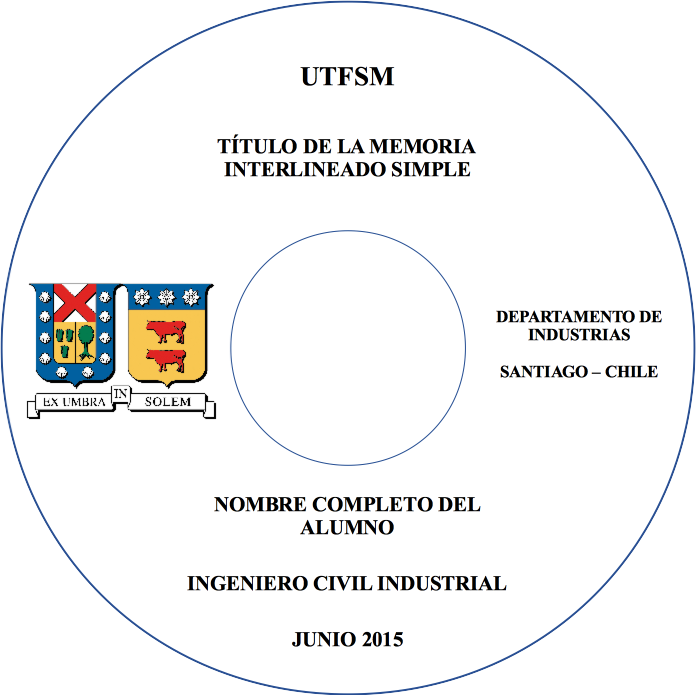
\includegraphics[width=.4\textwidth]{figures/thesis_cd.png}
\caption{Disco Compacto para Memoria UTFSM}
\label{fig:thesis_cd}
\end{figure}


Los CD se guardarán, en la biblioteca, en una caja de acrílico que tendrá una carátula de identificación dividida en tres franjas iguales, con las siguientes leyendas:
\begin{itemize}
		\item
    El escudo a color de la Institución de 20 mm de alto, centrado en la franja superior.
		\item
    El nombre completo del alumno, y centrado dos espacios más abajo el título de la memoria, en la franja del medio
		\item
    El nombre de la Unidad Académica, y renglón más abajo, año. En la franja inferior.
\end{itemize}


\begin{figure}[ht!]
\centering

\includegraphics[width=.4\textwidth]{figures/thesis_cd_cover.png}
\caption{Cubierta de Disco Compacto para Memorias y Tesis UTFSM.}
\label{fig:thesis_cd_cover}
\end{figure}


La carpeta \inlinecode{figures} incluye los diagramas (formato LibreOffice) para modificación e impresión.

%%%%%
\section{Documentos que se incluyen}

Se incluyen (en la carpeta \inlinecode{figures}) logotipos oficiales\footnote{Éstas son imágenes registradas y propiedad intelectual de la UTFSM y del Departamento de Industrias, y no están incluidas en la licencia de esta plantilla. La imagen corporativa de la UTFSM y del Departamento de Industrias están protegidas por leyes chilenas e internacionales de Derechos de autor. Su uso sólo está autorizado a estudiantes y memoristas de la UTFSM para fines de preparación de documentos académicos, incluidas memorias y tesis.}
de la UTFSM y del Departamento de Industrias.

\begin{figure}[ht!]
\centering

\includegraphics[scale = .5]{figures/logousm.png}
\caption{Logotipo de la UTFSM}
\label{fig:logousm}
\end{figure}

\begin{figure}[ht!]
\centering

\includegraphics[scale = .45]{figures/logousmleyenda.png}
\caption{Logotipo de la UTFSM (con leyenda)}
\label{fig:logousmleyenda}
\end{figure}


\begin{figure}[ht!]
\centering

\includegraphics[scale = .75]{figures/logousmind.jpg}
\caption{Logotipo de la UTFSM - Departamento de Industrias}
\label{fig:logousmind}
\end{figure}

\begin{figure}[ht!]
    \centering
    %\rule{4cm}{3cm}
    
\includegraphics[width=.8\textwidth]{figures/logo_utfsm_di.png}
    \caption{Logotipo del Departamento de Industrias, UTFSM (Formato lateral).}
    \label{fig:logodiutfsm}
\end{figure}

\begin{figure}[ht!]
\centering
%\rule{4cm}{3cm}

\includegraphics[width=.3\textwidth]{figures/logoind.png}
\caption{Logotipo del Departamento de Industrias, UTFSM }
\label{fig:logoind1}
\end{figure}


%%!TEX root = ../memoria.tex

\chapter{\LaTeX}


\section{Obtener \LaTeX{}}

\LaTeX{} es un sistema de preparación de documentos de alta calidad
visual \citep{latex:whatis}. Si no ha ocupado \LaTeX{} anteriormente,
visite esta página:
\begin{itemize}
\item \href{http://www.latex-project.org/}{http://www.latex-project.org/}
\end{itemize}
\begin{figure}[H]
\begin{centering}
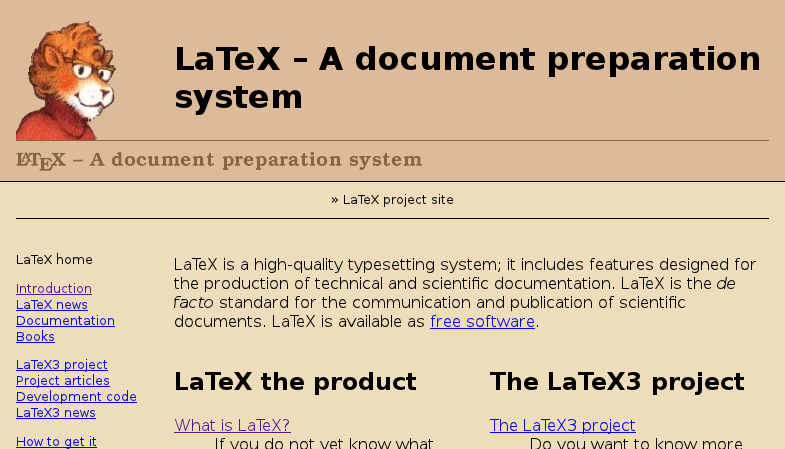
\includegraphics[width=0.7\textwidth]{figures/fig_latex_project_org}
\par\end{centering}

\caption{LaTeX Project}
\end{figure}


Puede obtener, en forma gratuita, las distribuciones de \LaTeX{},
según su plataforma, en:

\begin{description}
\item [Windows] \href{http://miktex.org/}{http://miktex.org/}; también puede
ocupar \href{http://www.tug.org/protext/}{http://www.tug.org/protext/}.

MikTex ofrece una versión básica. Después de instalarlo, asegúrese de descargar los paquetes adicionales requeridos para compilar esta plantilla.

\item [MacOS] \href{http://www.tug.org/mactex/}{http://www.tug.org/mactex/}.

La versión de MacTex es completa e incluye por defecto todos los paquetes necesarios para compilar esta plantilla.

\item [Unix/Linux] \href{http://www.tug.org/texlive/}{http://www.tug.org/texlive/}.

La instalación de TexLive en plataformas *nix es muy sencilla y directa a través de una consola (con permisos de administración):

(K/X)Ubuntu / Debian: \inlinecode{# apt-get install texlive}

Fedora: \inlinecode{# dnf install texlive}

RedHat / CentOS: \inlinecode{# yum install texlive}
\end{description}

Para una referencia completa sobre \LaTeX{}, recomendamos el libro
de \citealp{Lamport94}; aunque para solucionar problemas específicos,
su mejor aliado es Internet. Otros libros que puede consultar se presentan
en la Bibliografía \citep{Mittelbach04,Oetiker06,Roberts05,Borbon2014}.


\section{Editores para \LaTeX}
Existen muchos editores de \LaTeX, la mayoría de ellos de distribución gratuita y con versiones para los distintos sistemas operativos:
\begin{description}
    \item [TexStudio] Mac, Windows y Linux. \href{www.texstudio.org}{www.texstudio.org}.
    \item [TexMaker] Mac, Windows y Linux.  \href{www.xm1math.net/texmaker/}{www.xm1math.net/texmaker/}.
    \item[TeXworks] Mac, Window y Linux. \href{https://www.tug.org/texworks/}{https://www.tug.org/texworks/}
    \item [TexShop] Mac. \href{http://pages.uoregon.edu/koch/texshop/}{http://pages.uoregon.edu/koch/texshop/}.
    \item[Kile] Linux y Mac (vía macports). \href{http://kile.sourceforge.net/}{http://kile.sourceforge.net/}.
    \item[LaTeXila] Linux y Mac (vía Homebrew). \href{https://wiki.gnome.org/Apps/LaTeXila\#Installation}{https://wiki.gnome.org/Apps/LaTeXila\#Installation}.
\end{description}




%%%%%%%%%%%%%%%%%%%%%%%%%%%%%%%%%%%%%
%	Bibliografía
%%%%%%%%%%%%%%%%%%%%%%%%%%%%%%%%%%%%%
% \begin{spacing}{1}      % Single space for Bibliography
%    \bibliographystyle{thesis_utfsm}    % Alternative 'apalike'
%    \bibliography{bibliography}         % Archivo 'bibliography.bib'
% \end{spacing}


%%%%%%%%%%%%%%%%%%%%%%%%%%%%%%%%%%%%%
%	Anexos (Opcional)
%%%%%%%%%%%%%%%%%%%%%%%%%%%%%%%%%%%%%
% \appendix
% %!TEX root = memoria.tex
\chapter{LICENCIA}\label{appx:licencia}

{\footnotesize
\verbatiminput{LICENSE} 
}




\end{document}